% STEP 1: FORMAT-ONLY; not approved for submission.
% Original AAAI text is preserved in CONTENT_EXACT_FROM_AAAI.tex.
% Official MDPI ACS ZIP SHA-256: 62744425fbcec9cd3e58147cbee65bdec2e2ff0440f29792c26edc97a11b6c70
% Definitions/mdpi.cls v6.5a, 2026-09-11.
\documentclass[remotesensing,article,submit,moreauthors]{Definitions/mdpi}
\firstpage{1}
\makeatletter
\setcounter{page}{\@firstpage}
\makeatother
\pubvolume{1}
\issuenum{1}
\articlenumber{0}
\pubyear{2026}
\copyrightyear{2026}
\datereceived{ }
\daterevised{ }
\dateaccepted{ }
\datepublished{ }
\usepackage{algorithm}
\usepackage{algorithmic}
\usepackage{graphicx}
\usepackage{booktabs}
\usepackage{amsmath,amssymb}
% BG-REV: Toggle author-review markings (true) or clean submission text (false).
\usepackage{xcolor}
\newif\ifBGshowrevisions
\BGshowrevisionstrue
\DeclareRobustCommand{\BGRevAdd}[1]{\ifBGshowrevisions\begingroup\color{blue!70!black}#1\endgroup\else#1\fi}
\DeclareRobustCommand{\BGRevFigure}[1]{\ifBGshowrevisions\fcolorbox{blue!70!black}{white}{#1}\else#1\fi}

\newif\ifaaaiwithappendix
\aaaiwithappendixtrue
\newif\ifconditioncontractfigure
\IfFileExists{figures/figure3_condition_learning/figure3_condition_learning.pdf}
 {\conditioncontractfiguretrue}{\conditioncontractfigurefalse}
% BG-REV TITLE-PRIOR: author-approved title change from the historical AAAI source; see revision ledger.
\Title{Predicting the Background, Transporting the Structure: Decoupled Multimodal Subsurface Velocity Inversion}
\Author{Chunlei Wu, Yinghao Xu and Jing Lu*}
\AuthorNames{Chunlei Wu, Yinghao Xu and Jing Lu}
\address{[Author affiliations and numbering pending confirmation]}
\corres{Correspondence: [Jing Lu email pending confirmation]}
\abstract{
% BG-REV 2H-ABSTRACT: Entire revised scientific abstract is colored in marked mode.
\BGRevAdd{Subsurface velocity reconstruction from processed geophysical observations must reconcile complementary numerical and structural constraints: RMS velocity and sparse well logs inform broad velocity magnitudes, whereas post-stack time-migrated images and interpreted horizons delineate subsurface geometry. Conventional unified estimation does not explicitly assign these sources to background recovery and structure-bearing correction. We propose Physics-Decoupled Background-Guided Residual Flow Matching (PD-BG-RFM), a decoupled multimodal framework that learns background- and structure-oriented conditions while allowing every available modality to contribute to both. A deterministic branch predicts the smooth background velocity, and conditional Flow Matching generates the residual relative to that prediction, guided by structural conditions and an embedding of the predicted background. Crucially, the same background estimate defines residual supervision, vector-field conditioning, and final velocity composition. In full-field coordinates, this yields a transport path from an observation-dependent Gaussian reference centered on the predicted background toward the target velocity field. Exact composition and low-pass identities clarify the correction being modeled, while a necessary-and-sufficient condition characterizes when its straight-path target energy is lower than that of full-field transport. On 33,600 globally held-out OpenFWI-derived samples under a matched multimodal input and evaluation protocol, PD-BG-RFM achieves an RMSE of 0.0270, an SSIM of 0.9913, and a high-frequency MAE of 0.0065, leading the evaluated adapted baselines on these measures with 10.6 million trainable parameters. Controlled ablations, role-specific routing diagnostics, and transport-energy measurements further support the coordination of direct background estimation and conditional residual generation. The resulting reconstruction organization uses a shared predicted velocity background to connect heterogeneous geophysical evidence with structure-sensitive generative correction.}
}
% BG-REV 2H-KEYWORDS: Approved final scientific keywords, colored in marked mode.
\keyword{\BGRevAdd{seismic velocity model building; multimodal geophysical conditioning; conditional Flow Matching; deterministic background estimation; prediction-relative residual transport; processed seismic observations}}
% BG-REV 2H-HIGHLIGHTS: Author-approved MDPI two-question format, four complete blue bullets.
\addhighlights{yes}
\renewcommand{\addhighlights}{%
\begingroup\small
\noindent\textbf{What are the main findings?}
\begin{itemize}[topsep=0pt,itemsep=0pt]
% BG-REV 2H-HIGHLIGHTS-MF1
\item \BGRevAdd{Separating direct background prediction from conditional residual transport improves matched-input subsurface velocity reconstruction.}
% BG-REV 2H-HIGHLIGHTS-MF2
\item \BGRevAdd{On held-out OpenFWI-derived data, PD-BG-RFM leads the evaluated adapted baselines in RMSE, SSIM, and high-frequency MAE using 10.6M parameters.}
\end{itemize}
\noindent\textbf{What are the implications of the main findings?}
\begin{itemize}[topsep=0pt,itemsep=0pt]
% BG-REV 2H-HIGHLIGHTS-IM1
\item \BGRevAdd{The predicted background provides a shared numerical reference for residual supervision, transport conditioning, and model composition.}
% BG-REV 2H-HIGHLIGHTS-IM2
\item \BGRevAdd{Role-aware multimodal conditions link broad kinematic guidance and structural evidence while allowing each available modality to inform both routes.}
\end{itemize}
\endgroup
}
\reftitle{References}
\begin{document}
% BG-REV 2D-ENTRY: New active copy, old snapshots preserved.
% BG-REV 2D-TABLE1-FIT: Fit Table 1 inside the native text block; earlier content snapshot remains immutable.
% BG-REV 2E-ENTRY: Active Step 2E content; all prior snapshots remain immutable.
% BG-REV 2F-ENTRY: Active independent copy; all historical snapshots immutable.
% BG-REV 2G-ENTRY-C: Author-approved independent Step 2G snapshot.
% BG-REV 2H-ENTRY: Active Step 2H snapshot, prior stages immutable.


\begin{figure}[t]
\centering
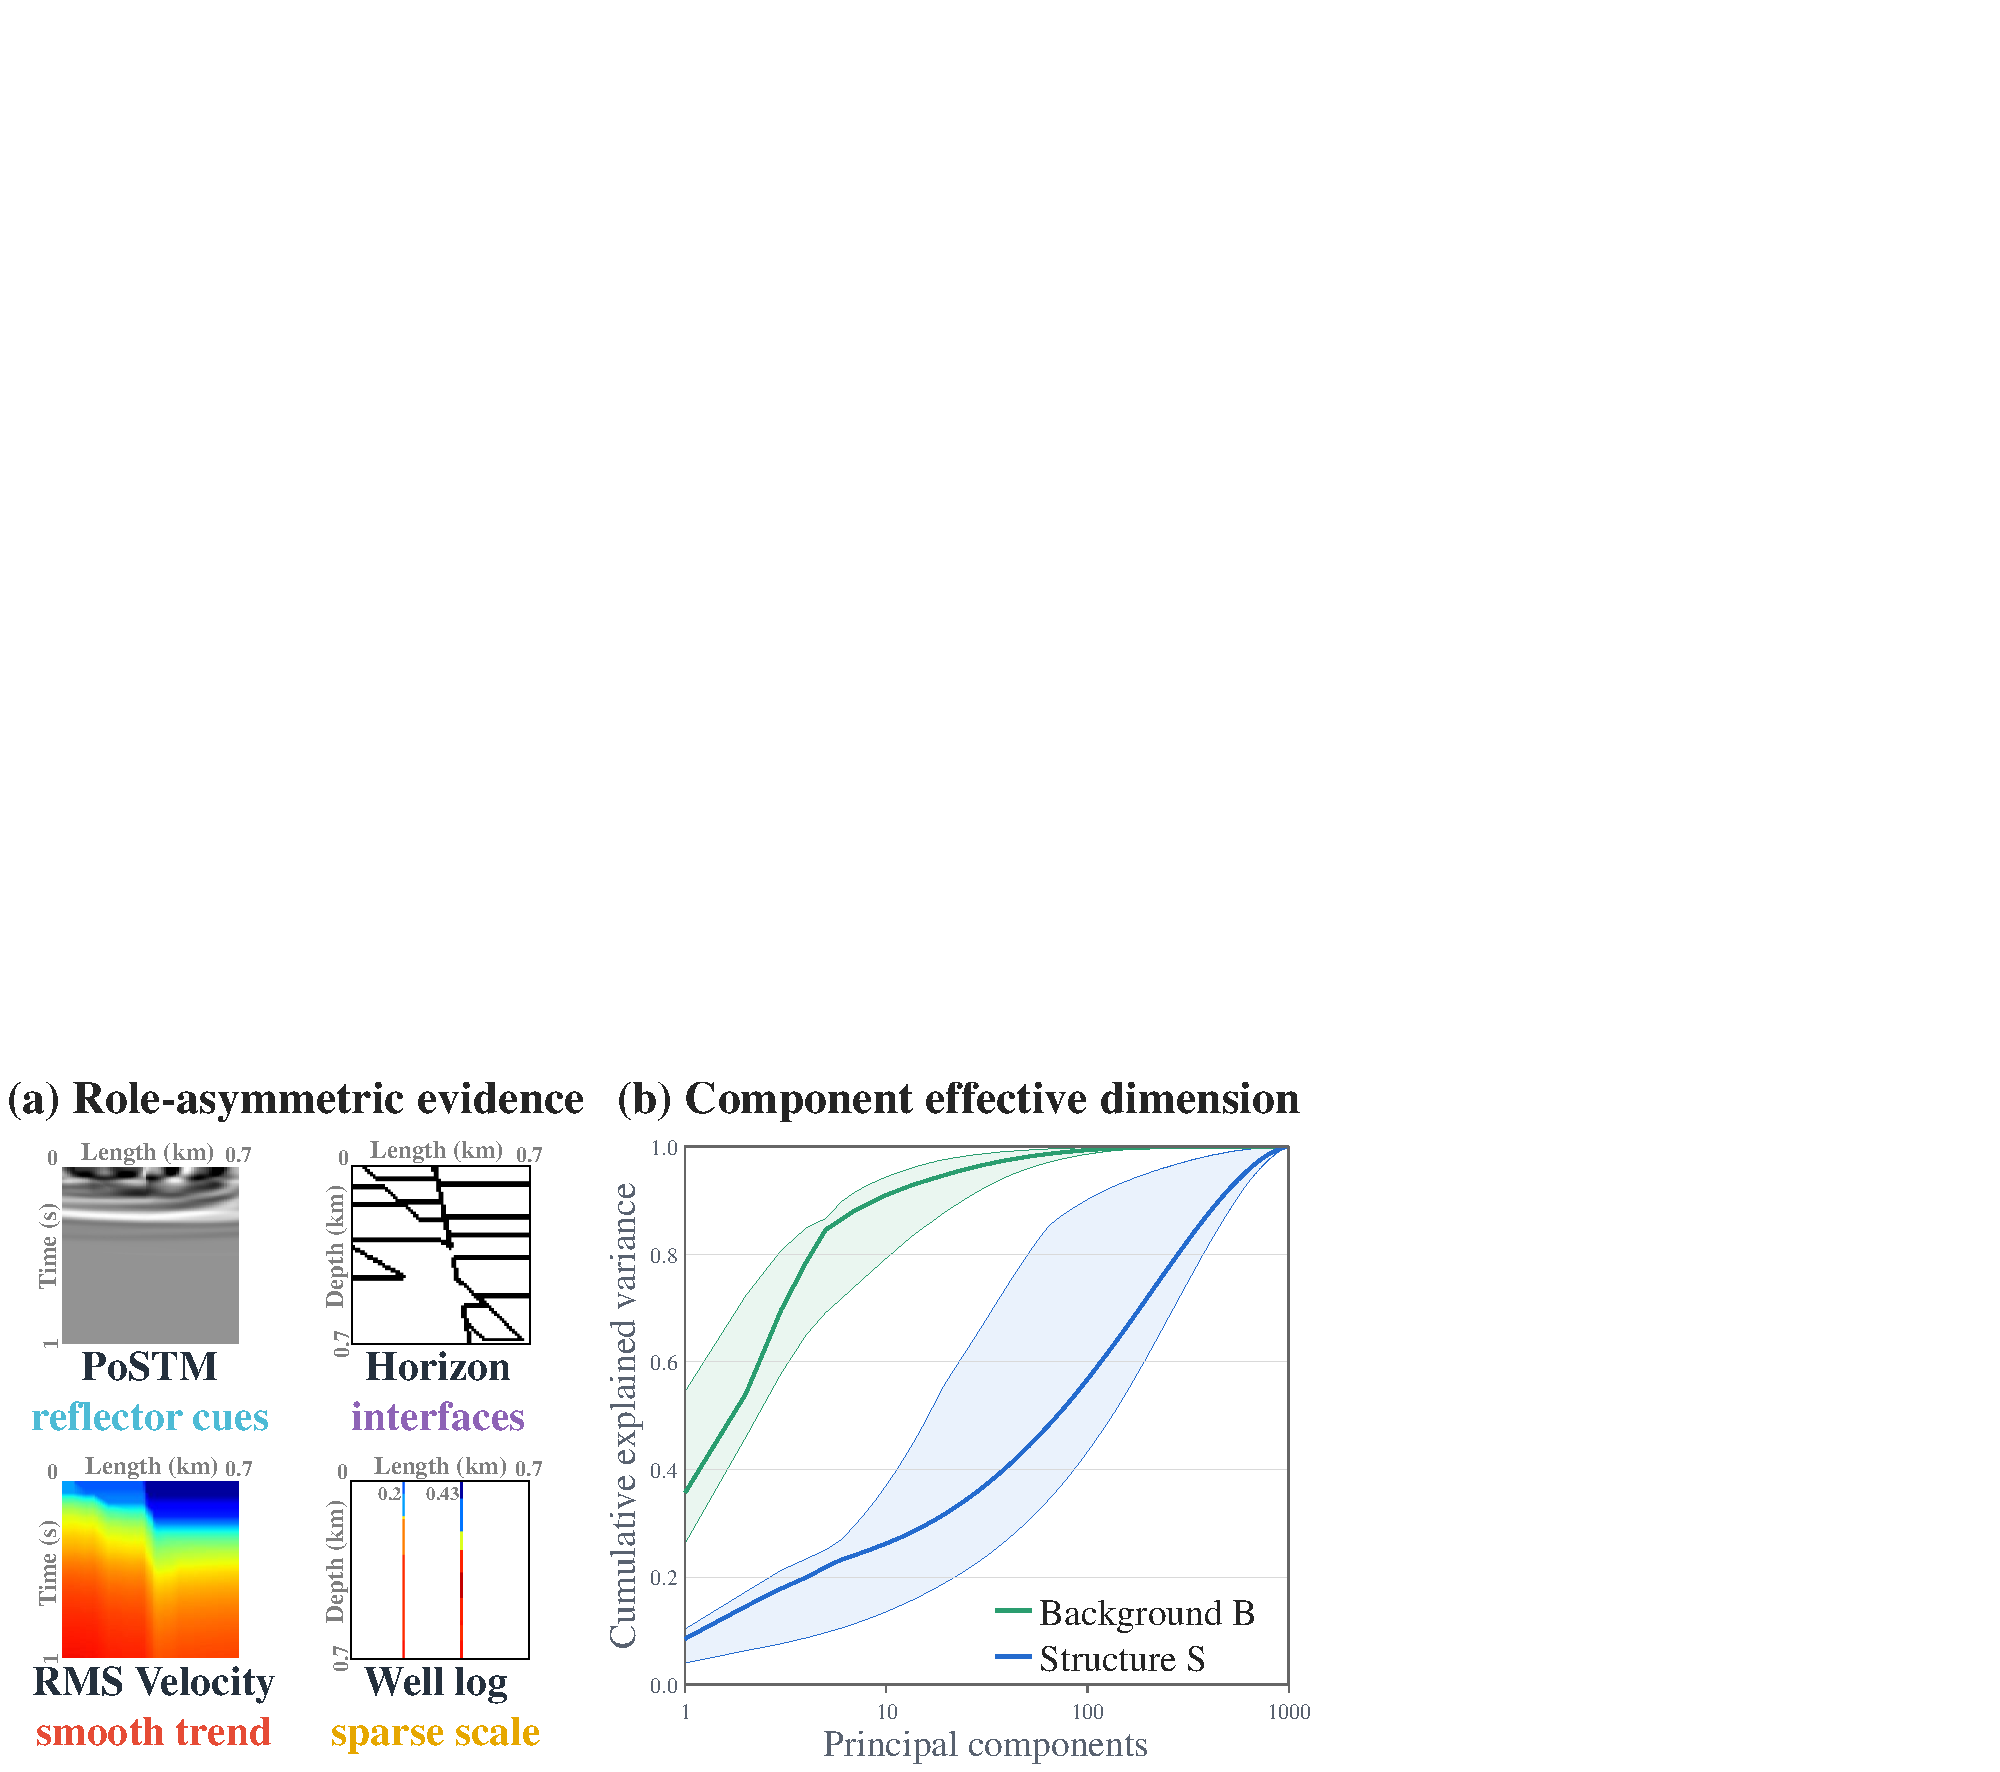
\includegraphics[width=0.98\columnwidth]{figures/aaai/motivation.pdf}
\caption{Data-level evidence for asymmetric conditional complexity. (a) Complementary geometry- and magnitude-oriented modality cues. (b) Cumulative PCA explained-variance curves across eight OpenFWI training subsets: background $B$ concentrates variance in fewer principal directions than structure $S$ (median effective rank $4.95$ versus $54.03$).}
\label{fig:motivation}
\end{figure}

\section{Introduction}

Subsurface velocity inversion estimates depth-domain velocity models for migration and structural interpretation \cite{stolt1978migration}. Classical full-waveform inversion (FWI) repeatedly solves the wave equation, but remains sensitive to initialization, acquisition coverage, cycle skipping, and computational cost \cite{tarantola1984inversion,bunks1995multiscale,pratt1998gaussnewton,virieux2009overview}. Learned inverse models amortize this mapping \cite{arayapolo2018deeptomography,yang2019deeplearning,wu2020inversionnet}, and OpenFWI provides large-scale benchmarks across velocity and fault families \cite{deng2022openfwi}. Practical model construction can also use post-stack migrated images (PoSTM), interpreted horizons, RMS velocity, and well logs \cite{stolt1978migration,dix1955velocities,hampson2001multiattribute}: the first two localize interfaces, while the latter constrain smooth trends and absolute scale.

% BG-REV 2F-INTRO-P2: Literature overview condensed to avoid overlap with Related Work.
\BGRevAdd{Learning-based velocity inversion encompasses direct regression from seismic records, physics-informed learning, and structured mappings between observational and model representations. These approaches use different training signals and observation protocols, so their architectures cannot be reduced to a single full-field design. Nevertheless, the choice of estimator does not by itself determine how heterogeneous evidence should be assigned to different reconstruction components. We return to these distinctions in Section~\ref{sec:related-work}.}

% BG-REV 2F-INTRO-P3: Literature overview condensed to avoid overlap with Related Work.
\BGRevAdd{Generative diffusion, score-based models, and Flow Matching extend velocity reconstruction beyond a single deterministic estimate by learning distributions or transport fields. Their relevance to subsurface inversion lies not only in the generative mechanism, but also in what is generated and which observations condition it. In a multimodal setting, transporting the entire velocity field can leave an informative background entangled with the structural correction, motivating a more explicit division of reconstruction responsibilities.}

% BG-REV 2F-INTRO-P4: Literature overview condensed to avoid overlap with Related Work.
\BGRevAdd{Multimodal representation learning provides mechanisms for aligning observations and coping with incomplete input sets. Such advances are important for combining seismic images, velocity trends, horizons, and well information, but representation alignment alone does not prescribe the role each condition should play in the reconstruction. The distinction between condition fusion and reconstruction-role allocation motivates the decoupled organization developed below.}

Early fusion permits role leakage, while full-field generation assigns one estimator to components of different conditional complexity. RMS velocity and sparse wells constrain much of the smooth background, whereas PoSTM and horizons primarily constrain the geometry of the remaining correction. The former is comparatively concentrated; the latter retains richer structural variability. We call this mismatch an \emph{asymmetry of conditional complexity}. Figure~\ref{fig:motivation} quantifies it using PCA \cite{jolliffe2002pca}: across all eight OpenFWI subsets, background $B$ concentrates variance in fewer directions than structure $S$, with median participation-ratio effective ranks of $4.95$ and $54.03$. This pronounced decomposition-specific degree-of-freedom gap motivates distinct estimator assignments, not simply a larger fused representation.

Frequency separation alone does not resolve the assignment. Oracle residualization creates a target shift: training uses $R_B=V-B$, but inference composes with $\hat B$, introducing a background mismatch $\hat B-B$ absent from supervision. The prediction-relative residual $R_{\hat B}=V-\hat B$ instead models the remaining \emph{structure-bearing variation} and any correction required for exact composition. Reusing $\hat B$ for residual supervision, conditioning, and composition defines \emph{prediction consistency}.

% BG-REV 2E-INTRO-P7: Refine original method-summary paragraph in full; author-review blue.
\BGRevAdd{We propose \emph{Physics-Decoupled Background-Guided Residual Flow Matching} (PD-BG-RFM), a decoupled multimodal inversion framework with role-aware conditions and distinct reconstruction responsibilities. Physics-decoupled contrastive learning uses subset-aware alignment, training-only wavelet anchors, cross-role separation, and reliability-weighted fusion to construct background-oriented and structure-oriented conditions from every available modality, without hard-assigning observations to routes. The background branch deterministically predicts $\hat B$; the same prediction defines the residual target $V-\hat B$, conditions residual transport jointly with $C_{\mathrm{str}}$, and is added back to compose the final estimate. This yields the block-triangular contract $C_{\mathrm{bg}}\mapsto\hat B$ and $(C_{\mathrm{str}},\hat B)\mapsto\hat R$, linking representation roles to generation responsibilities. The interfaces are learned jointly, but the generator-facing dependence flows only from the predicted background into the residual route. We derive exact composition and low-pass identities and characterize when this routing lowers straight-path target energy.}

Our contributions are threefold:
\begin{itemize}
% BG-REV 2E-INTRO-C1: Refine first contribution bullet in full; author-review blue.
\item \BGRevAdd{We identify an asymmetry of conditional complexity and formalize role-aware multimodal conditioning through the block-triangular contract $C_{\mathrm{bg}}\mapsto\hat B$ and $(C_{\mathrm{str}},\hat B)\mapsto\hat R$. Both routes encode available modalities, while the background prediction provides one-way context for residual transport.}
\item We introduce prediction-consistent residual Flow Matching, reusing one background prediction for residual supervision, vector-field conditioning, and final composition. This shared reference removes background mismatch from composition error by construction.
\item We derive exact composition-consistency and low-pass-burden identities and prove a necessary-and-sufficient condition for residual transport to have lower straight-path target energy than full-field transport.
\end{itemize}
On globally held-out OpenFWI examples, PD-BG-RFM achieves the best matched-input RMSE, SSIM, and high-frequency MAE with only 10.6M parameters. This compact design assigns deterministic prediction to the background and residual transport to the prediction-relative correction. Controlled ablations and branch-specific diagnostics test whether its performance and efficiency follow from the proposed condition interfaces and responsibility allocation.

\begin{figure*}[t]
\centering
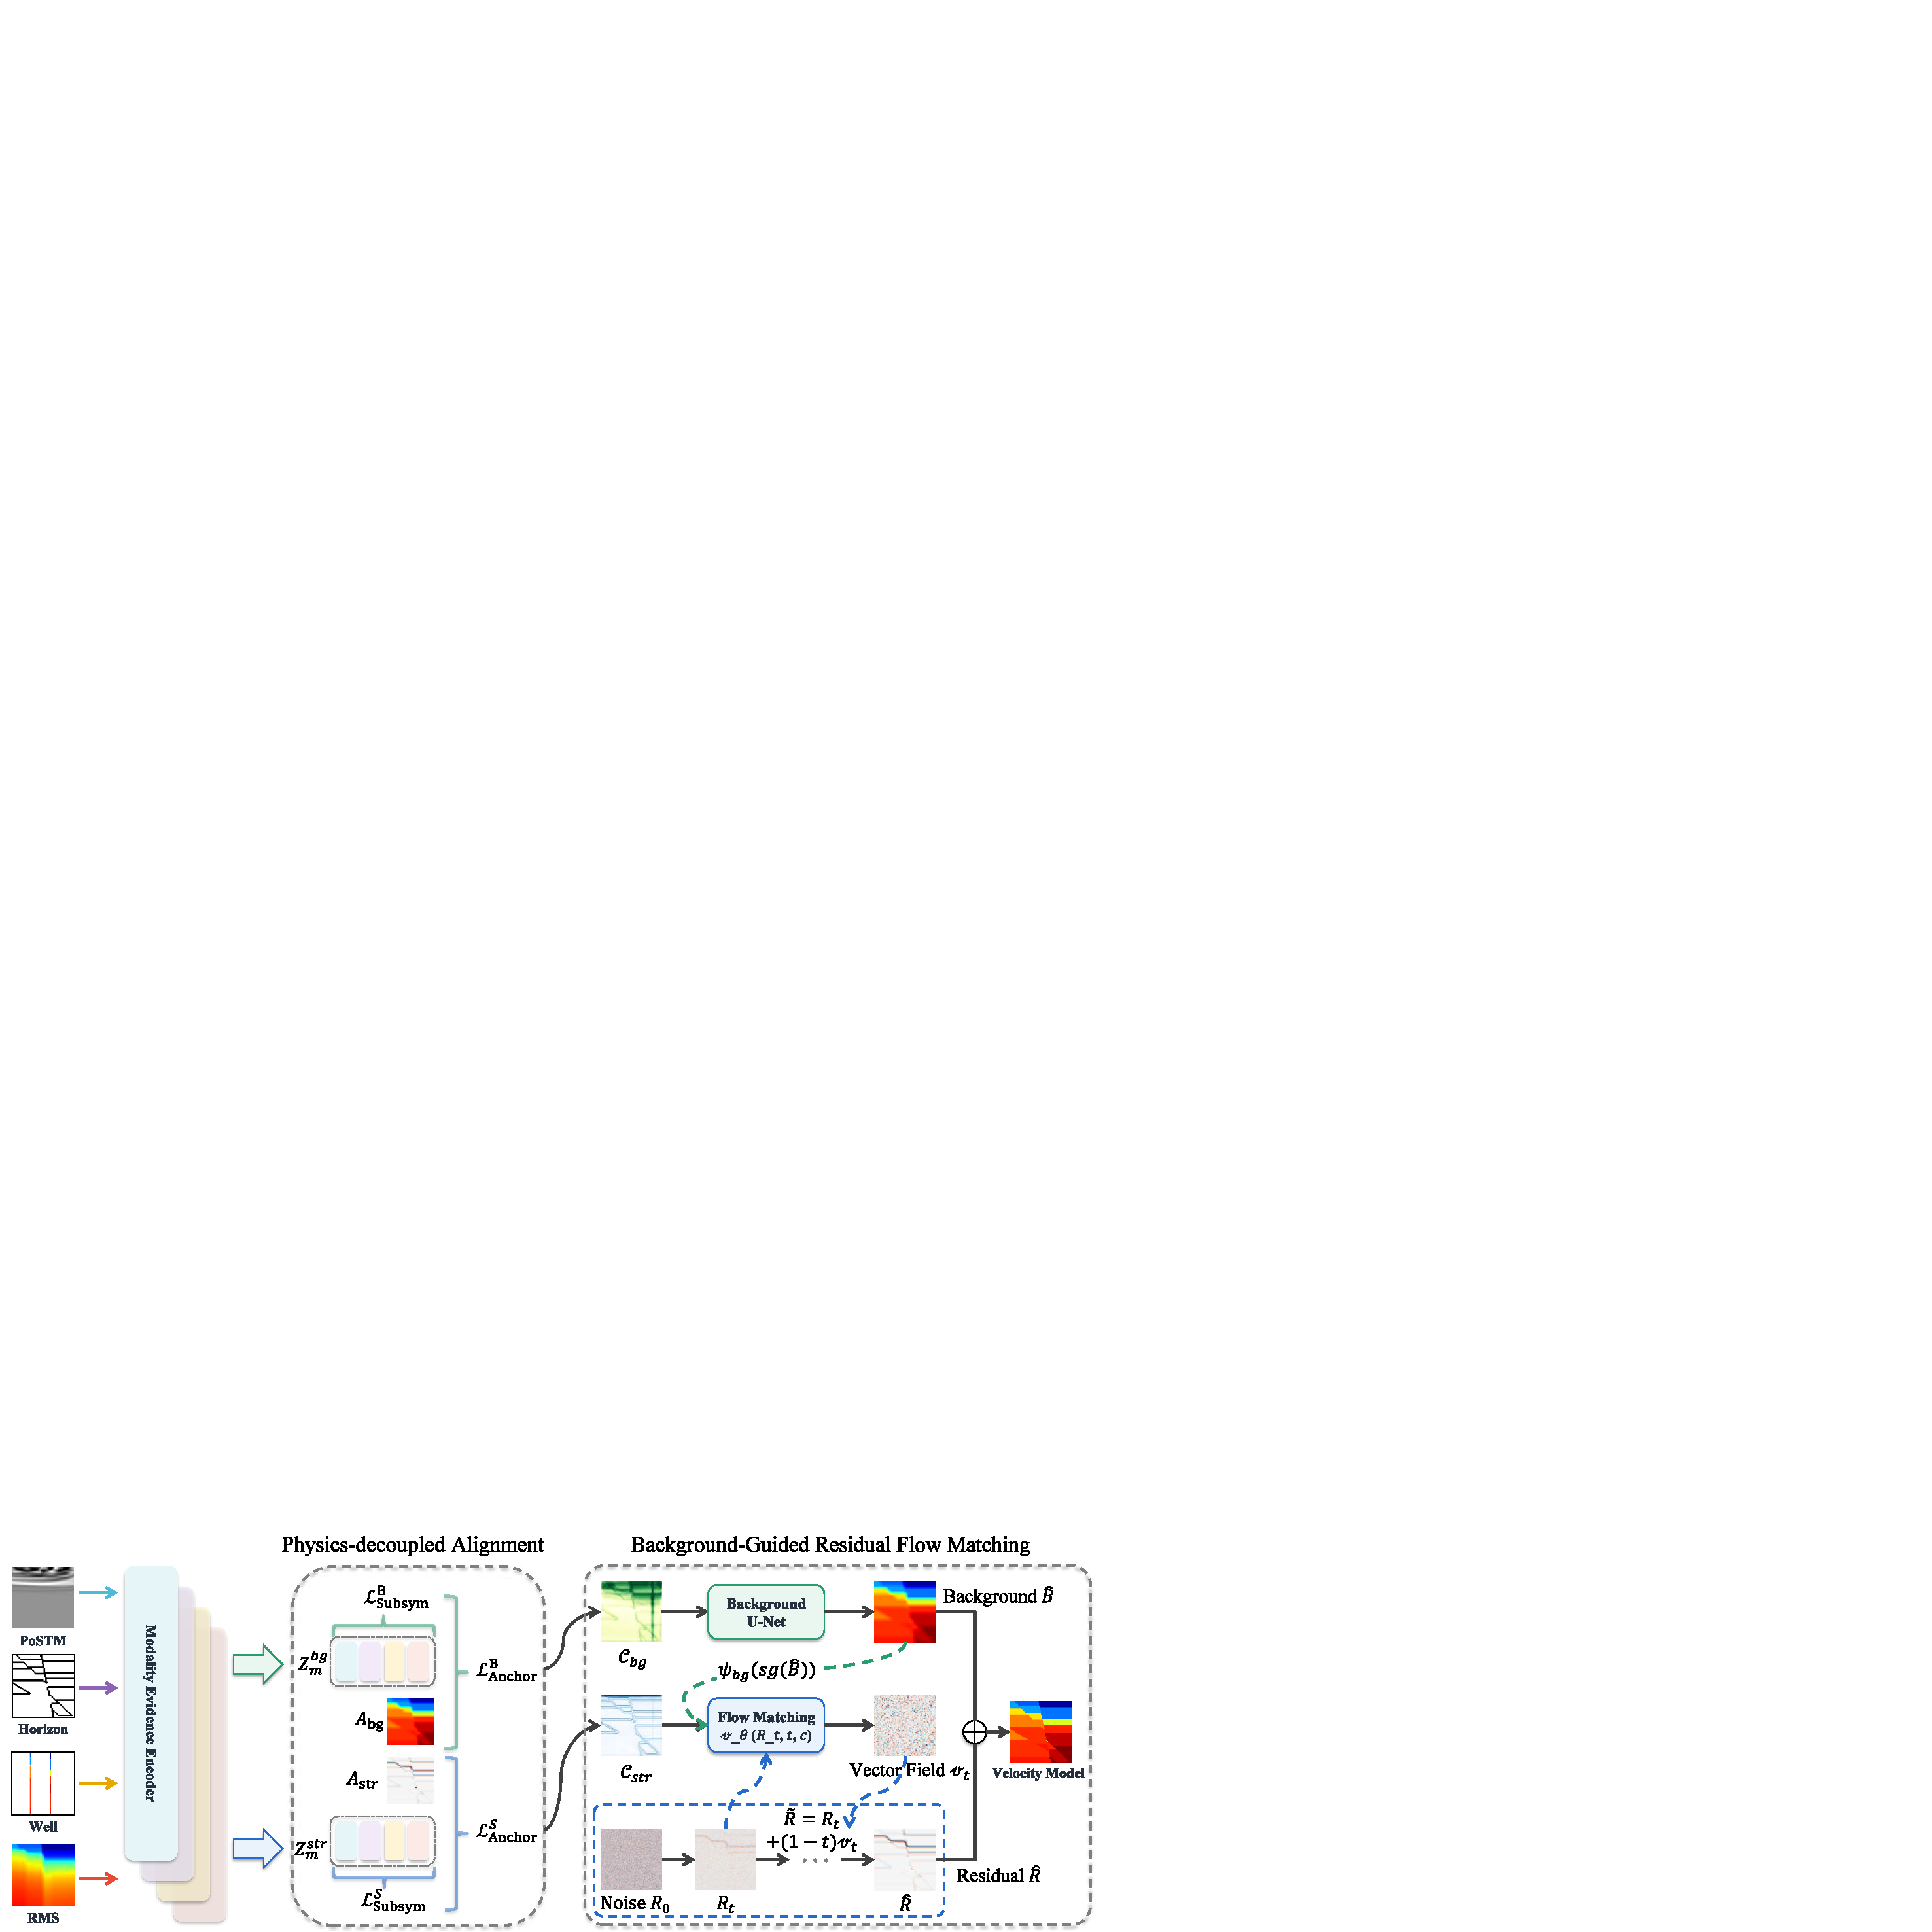
\includegraphics[width=0.98\textwidth]{figures/aaai/method_overview.pdf}
\caption{PD-BG-RFM and its physics-decoupled condition contract. Dashed orange paths provide training supervision; solid paths form inference. The background prediction defines the residual target, conditions transport, and composes the output.}
\label{fig:method-overview}
\end{figure*}

% BG-REV 2F-H-RELATED-WORK: New, independent Related Work section.
\section{Related Work}
\label{sec:related-work}

% BG-REV 2F-RW-S1: New subsection heading.
\subsection{Learning-Based Seismic Velocity Inversion}

% BG-REV 2F-RW-S1-P1: New academic paragraph in author-review blue.
\BGRevAdd{Learning-based seismic velocity inversion replaces part of the iterative model-updating process with an estimated mapping from observations to subsurface velocity. Direct convolutional approaches demonstrated this possibility using seismic shot records: fully convolutional inversion and InversionNet learn supervised waveform-to-velocity mappings, while OpenFWI provides controlled families of layered and faulted velocity models for evaluating such estimators \cite{yang2019deeplearning,wu2020inversionnet,deng2022openfwi}. Dense encoder--decoder variants such as SVInvNet extend this direct-estimation line \cite{najafi2025svinvnet}. These advances establish the effectiveness of amortized inversion, but the source information remains essential to interpreting their results. A network trained on multi-shot waveforms solves a different observation problem from one receiving processed RMS velocity, migrated sections, interpreted horizons, and sparse well ties. Numerical comparisons across these settings must therefore distinguish the information supplied to the estimator from its prediction architecture.}

% BG-REV 2F-RW-S1-P2: New academic paragraph in author-review blue.
\BGRevAdd{Other work alters the relationship between learning and physical modeling rather than simply enlarging a convolutional inverse. UPFWI couples a convolutional representation with wave-equation consistency in an unsupervised loop \cite{jin2022upfwi}, whereas physics-informed networks use physical constraints to shape the learned solution \cite{rashtbehesht2022pinn}. Auto-Linear investigates structured latent relations between subsurface forward and inverse problems \cite{feng2024autolinear}, and the unified latent-translation framework of Gupta et al.\ studies forward and inverse mappings in a shared representation \cite{gupta2025gfi}. These approaches illustrate materially different supervision and representation choices, not interchangeable full-field regressors. Their central concern is how to estimate or relate seismic and velocity quantities; they do not directly impose the background-to-residual generation responsibility used here.}

% BG-REV 2F-RW-S1-P3: New academic paragraph in author-review blue.
\BGRevAdd{Processed-constraint reconstruction has a separate lineage closer to interpretation-guided model building. Kim et al.\ combine a low-resolution velocity model, a migration image, a well-derived prior, and a reliability-weight map to refine velocity resolution \cite{kim2024resolution}. More recently, Wu et al.\ use masked-autoencoder representations of migration results and an initial velocity model, followed by seismic--well calibration, for three-dimensional velocity refinement including field data \cite{wu2026seismicwell}. Their reconstruction inputs and field-oriented protocols should not be conflated with waveform-based OpenFWI inversion or the present synthetic constraint setting. PD-BG-RFM differs from these learned reconstruction workflows primarily in its explicit division of the estimation task: it predicts a smooth background directly and assigns conditional generative transport to the correction relative to that prediction.}

% BG-REV 2F-RW-S2: New subsection heading.
\subsection{Generative Models for Subsurface Reconstruction}

% BG-REV 2F-RW-S2-P1: New academic paragraph in author-review blue.
\BGRevAdd{Generative modeling changes the inverse problem from predicting a single map to learning how plausible models are represented or sampled under observations. Denoising diffusion and score-based formulations progressively recover samples from noise, while latent diffusion performs this operation in a learned representation to reduce the dimensional burden \cite{ho2020ddpm,song2021scorebased,rombach2022ldm}. For inverse problems, posterior-sampling methods combine learned generative priors with measurement information \cite{chung2023diffusionposterior}. These methods differ in how they enforce observation agreement and in whether sampling takes place in the ambient model domain or in a latent space. Thus, using diffusion is not itself a definition of the geophysical reconstruction target, nor does a generative sampler automatically resolve disagreements between heterogeneous conditions.}

% BG-REV 2F-RW-S2-P2: New academic paragraph in author-review blue.
\BGRevAdd{In subsurface applications, controllable seismic velocity synthesis demonstrates conditional generation under geological or well-related information \cite{wang2024controllable}, while WaveDiffusion models a joint latent representation for seismic and velocity generation \cite{wang2024wavediffusion}. DiffusionVel combines separate seismic-conditioned, well-conditioned, and geology-oriented diffusion components, with low-pass background information incorporated during sampling \cite{zhang2024diffusionvel}. Zhang et al.\ also investigate diffusion-based initial velocity construction constrained by well data and migration-derived structural information for subsequent full-waveform inversion \cite{zhang2025wellstructure}. These studies show that background information and structural observations can enter generative workflows in distinct ways. They do not, however, imply a common residual target, a shared background estimator, or an identical route by which prediction error is handled at composition.}

% BG-REV 2F-RW-S2-P3: New academic paragraph in author-review blue.
\BGRevAdd{Flow Matching offers another mechanism for learning continuous transport through vector-field regression \cite{lipman2023flowmatching,liu2023rectifiedflow}, related to dynamic transport formulations \cite{benamou2000computational}. PD-BG-RFM adopts this established framework without proposing a new class of transport dynamics. Its distinction lies instead in organizing the transported quantity and the conditioning reference: a deterministic branch first predicts $\hat B$, and the Flow Matching target is defined relative to that same prediction rather than to an oracle background or to the full velocity field. The predicted background also conditions the vector field and is reused when composing the final velocity. This design separates direct estimation of the smoother component from conditional generation of the structure-bearing correction, while leaving the accuracy of both components an empirical matter.}

% BG-REV 2F-RW-S3: New subsection heading.
\subsection{Multimodal Geophysical Conditioning}

% BG-REV 2F-RW-S3-P1: New academic paragraph in author-review blue.
\BGRevAdd{Geophysical constraints differ in what they measure, where they are sampled, and how directly they inform velocity. RMS velocity carries time-domain kinematic and magnitude information, whereas post-stack migrated images emphasize reflector geometry; interpreted horizons supply explicit stratigraphic boundaries, and sparse well logs constrain velocity locally \cite{dix1955velocities,stolt1978migration,hampson2001multiattribute}. These inputs are complementary rather than exchangeable. For example, the low-resolution velocity, migration, well prior, and reliability map used by Kim et al.\ provide different forms of numerical and structural guidance \cite{kim2024resolution}; well- and structure-constrained diffusion similarly uses distinct observations to shape initial models \cite{zhang2025wellstructure}. Their use illustrates why a single notion of measurement confidence is insufficient to specify every modality's contribution to reconstruction.}

% BG-REV 2F-RW-S3-P2: New academic paragraph in author-review blue.
\BGRevAdd{Multimodal learning has developed methods for aligning complementary views and retaining information when inputs are incomplete \cite{baltrusaitis2019multimodal}. Contrastive representation learning exploits correspondence between paired views \cite{tian2020cmc,radford2021clip}; Symile extends contrastive agreement to tuples of modalities \cite{saporta2024symile}, and HeMIS addresses heterogeneity and missing-modality observations \cite{havaei2016hemis}. Shared/private representation objectives can also discourage information from unrelated roles being mixed indiscriminately \cite{bousmalis2016domain}. These tools act principally on the learned condition space: they help answer whether heterogeneous inputs can be represented together, which information is available, and which alignments should be retained. The downstream question of whether a learned condition should drive background prediction or structural correction remains separate.}

% BG-REV 2F-RW-S3-P3: New academic paragraph in author-review blue.
\BGRevAdd{Reliability-aware fusion provides a further degree of control, but weighting observations is not equivalent to assigning reconstruction responsibilities. A reliability-weight map can encode confidence in a well-derived prior \cite{kim2024resolution}; learned feature weights can also adjust contributions according to input quality or context. PD-BG-RFM combines role-aware representations with separately fused background- and structure-oriented conditions. Crucially, each available modality may inform both conditions, while the deterministic background estimate enters residual transport as a shared prediction reference. The learned routing weights therefore describe a conditional allocation induced by the training objectives and reliability priors, not an autonomous discovery of uniquely identifiable physical factors. The distinction is between \emph{how} heterogeneous evidence is fused and \emph{what part of the velocity reconstruction} each fused condition is asked to support.}

% BG-REV 2D-H-METHOD: Rename Method to Materials and Methods.
\section{Materials and Methods}

\BGRevAdd{This study considers subsurface velocity reconstruction from geophysical constraints that are available after seismic processing or interpretation, rather than directly from shot gathers. The observations comprise post-stack time-migrated (PoSTM) sections and root-mean-square (RMS) velocity fields, both sampled on a $1000\times70$ time--lateral grid, together with horizon maps and sparse well-velocity constraints represented on a $70\times70$ depth--lateral grid. The reconstruction target is a velocity model defined on the same depth grid. These sources provide complementary information about reflector geometry, propagation kinematics, geological interfaces, and local velocity control, while differing in their physical meaning and sampling domains. The problem addressed here is therefore how to organize such heterogeneous, precomputed observations for velocity reconstruction.}

\subsection{The Physics-Decoupled Condition Contract}
Let $X_\Omega=\{x_m:m\in\Omega\}$ be the observed subset, with $\Omega\subseteq\mathcal M$ and $\mathcal M=\{\mathrm{PoSTM},\mathrm{Horizon},\mathrm{RMS},\mathrm{Well}\}$, and let $V\in\mathbb R^{H\times W}$ be the target velocity model. We assign deterministic prediction to background velocity and generative transport to the remaining structure-bearing variation. PoSTM and horizons predominantly localize geometry, whereas RMS velocity and wells calibrate magnitude \cite{stolt1978migration,dix1955velocities,hampson2001multiattribute}; these are tendencies, not a hard modality partition, so both roles encode every available modality. We implement $P_L$ as linear stride-one average pooling and set $P_H=I-P_L$:
\begin{equation}
B=P_L(V),\qquad S=P_H(V),\qquad V=B+S.
\label{eq:frequency-view}
\end{equation}
$S$ is the complementary component induced by smoothing and is used for training and diagnosis. The transported variable is instead the prediction-relative residual $R_{\hat B}=V-\hat B$, which generalizes $S$ by including the background correction required for exact composition.

\paragraph{Definition 1 (Physics-decoupled condition contract).}
Let $b$ and $r$ denote the background and residual variables, and let $\psi_{\mathrm{bg}}$ be a learned convolutional embedding of a background field. We define the contract as the following block-triangular conditional factorization:
\begin{equation}
\begin{aligned}
(C_{\mathrm{bg}},C_{\mathrm{str}})&=E_\phi(X_\Omega),\\
p_{\mathrm{PD}}(b,r\mid X_\Omega)
&=\delta_{f_{\mathrm{bg}}(C_{\mathrm{bg}})}(b)
\,p_\theta(r\mid C_{\mathrm{str}},\psi_{\mathrm{bg}}(b)).
\end{aligned}
\label{eq:asymmetric-factorization}
\end{equation}
The estimate is $\hat V=\hat B+\hat R$, where $\hat B=f_{\mathrm{bg}}(C_{\mathrm{bg}})$ and $\hat R\sim p_\theta(\,\cdot\mid C_{\mathrm{str}},\psi_{\mathrm{bg}}(\hat B))$. Thus $C_{\mathrm{bg}}$ is the interface for deterministic background prediction, while $C_{\mathrm{str}}$ and the predicted background jointly condition structure-bearing residual generation. The one-way dependence from the background route to the residual route makes the factorization block triangular, without imposing a hard modality partition inside $E_\phi$. The Dirac measure encodes this architectural point-estimator assignment, not a degenerate true posterior, frequency--uncertainty equivalence, or identifiable representation. Figure~\ref{fig:method-overview} summarizes the contract and computation graph.

\subsection{Instantiating the Condition Contract}
In Definition~1, $E_\phi$ is the complete condition-learning stack: modality subencoders, role-aware fusion, and internal role adapters. Each $\mathcal E_{\phi,m}(x_m)=(Z_m^{\mathrm{bg}},Z_m^{\mathrm{str}},r_m)$ uses a convolutional backbone on the velocity grid, lightweight $1\times1$ role heads, and a reliability head $r_m=(r_m^{\mathrm{bg}},r_m^{\mathrm{str}})$. Physics-decoupled contrastive learning calibrates these features and routes while retaining every modality in both roles. The fusion and adapters below therefore belong to $E_\phi$, rather than forming extra condition modules, and are optimized jointly as one condition mapping. A training-only auxiliary separation regularizer does not create a third interface or enter either generator; full details appear in Appendix~\ref{app:condition-objective}.

Suppressing the sample index, let $a_m\in\{0,1\}$ and $q_m\in[0,1]$ denote availability and external quality, with $\Omega=\{m:a_m=1\}$. Role-aware fusion forms
\begin{align}
\bar C_k
&=\sum_{m\in\Omega}w_m^k Z_m^k,
\qquad k\in\{\mathrm{bg},\mathrm{str}\},\nonumber\\
C_{\mathrm{bg}}&=\bar C_{\mathrm{bg}},\qquad
C_{\mathrm{str}}=g_{\mathrm{str}}(\bar C_{\mathrm{str}}).
\label{eq:reliability-fusion}
\end{align}
Here the background adapter is the identity, whereas $g_{\mathrm{str}}$ is a lightweight spatial adapter that produces the generator's structural condition; the two interfaces may have different channel counts. The normalized $w_m^k$ combines availability $a_m$, externally supplied quality $q_m$, and predicted role reliability $r_m^k$, assigning zero weight to unavailable modalities. In our OpenFWI protocol $q_m=a_m$, and no target-derived statistic enters fusion; Appendix~\ref{app:condition-objective} restores the sample index and gives the complete normalization.

Training-only Haar anchors $A_{\mathrm{bg}}=W_L(V)$ and $A_{\mathrm{str}}=W_H(V)$ \cite{mallat1989theory} calibrate the two roles: the former is the resized approximation band and the latter combines detail bands. They differ from the average-pooled background target $B$ and are unavailable at inference. The active condition objective is
\begin{align}
\mathcal L_C
={}&\mathcal L_{\mathrm{subsym}}^{\mathrm{bg}}
 +\mathcal L_{\mathrm{subsym}}^{\mathrm{str}}+\lambda_A\mathcal L_A
 +\lambda_{\mathrm{bg,str}}\mathcal L_{\mathrm{bg,str}}^{\perp}
\nonumber\\
&+\lambda_{\mathrm{aux}}\mathcal L_{\mathrm{aux}}^{\perp}
 +\lambda_Q\mathcal L_{\mathrm{rel}}.
\label{eq:condition-loss}
\end{align}
\BGRevAdd{Role-aware condition learning combines cross-modal alignment with complementary supervision for the two reconstruction roles. Within each group of samples sharing the same set of available modalities, Subset-Symile contrasts aligned representations from the same training record, together with the corresponding role anchor, against tuples constructed by within-group derangements \cite{saporta2024symile}. The role-specific anchors are derived from a one-level Haar decomposition of the reference velocity: the approximation component provides a numerical, background-oriented reference, whereas the aggregated detail components provide a structure-oriented reference \cite{mallat1989theory}. Anchor calibration encourages the projected modality representations to agree with these references, while the orthogonality terms discourage redundancy among the learned role representations. Reliability weighting further regulates the contributions of available modalities without assigning any observation exclusively to either reconstruction branch. Together, these mechanisms encourage the background- and structure-oriented conditions to retain complementary information for deterministic background estimation and prediction-relative residual transport, respectively. The reference-derived anchors are used exclusively during training and are not required at inference. Complete definitions of the auxiliary objectives and fusion normalization are provided in Appendix~\ref{app:condition-objective}.}


\begin{algorithm}[!b]
	\caption{Training procedure for PD-BG-RFM under the backward contract}
	\label{alg:pdbg-rfm}
	\textbf{Input}: batch $\mathcal B=(X_\Omega,V,a,q)$\\
	\textbf{Parameters}: $\Theta=(\phi,\omega_{\mathrm{bg}},\theta)$\\
	\textbf{Output}: updated parameters $\Theta$
	\begin{algorithmic}[1]
		\STATE \textbf{I. Learn physics-decoupled conditions.}
		\STATE $\{Z_m^{\mathrm{bg}},Z_m^{\mathrm{str}},r_m\}_{m\in\Omega}\gets\{\mathcal E_{\phi,m}(x_m)\}_{m\in\Omega}$.
		\STATE $(\bar C_{\mathrm{bg}},\bar C_{\mathrm{str}})\gets\operatorname{Fuse}_{a,q,r}(\{Z_m^{\mathrm{bg}},Z_m^{\mathrm{str}}\}_{m\in\Omega})$.
		\STATE $C_{\mathrm{bg}}\gets\bar C_{\mathrm{bg}}$; $C_{\mathrm{str}}\gets g_{\mathrm{str}}(\bar C_{\mathrm{str}})$.
		\STATE $(A_{\mathrm{bg}},A_{\mathrm{str}})\gets(W_L(V),W_H(V))$; compute $\mathcal L_C$ by Eq.~\ref{eq:condition-loss}.
		\STATE \textbf{II. Predict background velocity deterministically.}
		\STATE $\hat B\gets f_{\mathrm{bg}}(C_{\mathrm{bg}})$; compute $\mathcal L_{\mathrm{bg}}$ by Eq.~\ref{eq:background-loss}.
		\STATE $\bar B\gets\operatorname{sg}[\hat B]$; $R_{\hat B}\gets V-\bar B$.
		\STATE \textbf{III. Transport the prediction-consistent residual.}
		\STATE Sample $t\sim\mathcal U(0,1)$ and $\xi\sim\mathcal N(0,I)$.
		\STATE $c\gets[C_{\mathrm{str}};\psi_{\mathrm{bg}}(\bar B)]$; $R_t\gets(1-t)\xi+tR_{\hat B}$.
		\STATE $u_t\gets R_{\hat B}-\xi$; $\widehat u_t\gets v_\theta(R_t,t,c)$.
		\STATE $\widetilde R\gets R_t+(1-t)\widehat u_t$; compute $\mathcal L_R$ by Eq.~\ref{eq:residual-loss}.
		\STATE \textbf{IV. Optimize under the backward contract.}
		\STATE $\mathcal L\gets\mathcal L_R+\mathcal L_{\mathrm{bg}}+\lambda_C\mathcal L_C$.
		\STATE $\Theta\gets\operatorname{OptStep}(\Theta,\nabla_\Theta\mathcal L)$.
		\STATE \textbf{return} $\Theta$
	\end{algorithmic}
\end{algorithm}


\subsection{Background-Guided Residual Flow Matching}
A full-resolution U-Net \cite{ronneberger2015unet} with parameters $\omega_{\mathrm{bg}}$ deterministically predicts $\hat B=f_{\mathrm{bg}}(C_{\mathrm{bg}})$ on the same spatial grid as $V$, under
\begin{equation}
\mathcal L_{\mathrm{bg}}
=
\|\hat B-P_L(V)\|_1+\lambda_{\mathrm{bg},2}\|\hat B-P_L(V)\|_2^2.
\label{eq:background-loss}
\end{equation}
The prediction is reused throughout the pipeline: it defines residual supervision, joins $C_{\mathrm{str}}$ as context, and is added back for final composition. We therefore define
\begin{equation}
R_{\hat B}=V-\hat B,
\label{eq:prediction-consistent-residual}
\end{equation}
rather than the oracle residual $R_B=V-B$. Using the same $\hat B$ for supervision, context, and composition aligns the residual task encountered during training and inference. We call this construction \emph{prediction-consistent residual transport}; Theorem~1 characterizes it.


% BG-REV 2D-TABLE1-FIT: Table 1 presentation-only width correction; all original cells retained.
\begin{table*}[t]
\begin{adjustwidth}{0cm}{0cm}
	\centering
	% PD-BG-RFM values come from the verified global-held-out final-checkpoint artifact.
	% AAAI permits 9pt tables when the normal 10pt size does not fit.
	\small
	\setlength{\tabcolsep}{2pt}
	\resizebox{\linewidth}{!}{%
\begin{tabular}{@{}c c c c c c c c c@{}}
		\toprule
		Dataset & Metric & InversionNet & VelocityGAN & UPFWI & Auto-Linear & \shortstack{Invertible\\X-Net} & \shortstack{Latent U-Net\\(Large)} & \textbf{PD-BG-RFM} \\
		\midrule
		\multicolumn{2}{c}{\shortstack{Method paper}} & \multicolumn{2}{c}{\shortstack{NeurIPS 2022\\\cite{deng2022openfwi}}} & \shortstack{ICLR 2022\\\cite{jin2022upfwi}} & \shortstack{ICML 2024\\\cite{feng2024autolinear}} & \multicolumn{2}{c}{\shortstack{ICLR 2025\\\cite{gupta2025gfi}}} & \shortstack{\textbf{Ours}} \\
		\midrule
		& MAE $\downarrow$ & 0.0143 & 0.0118 & 0.0621 & \underline{0.0081} & 0.0159 & \textbf{0.0060} & 0.0087 \\
		FlatVel-A & RMSE $\downarrow$ & 0.0257 & 0.0178 & 0.1233 & 0.0224 & 0.0235 & \textbf{0.0098} & \underline{0.0138} \\
		& SSIM $\uparrow$ & 0.9909 & 0.9916 & 0.9565 & 0.9888 & 0.9917 & \textbf{0.9967} & \underline{0.9961} \\
		\addlinespace[2pt]
		& MAE $\downarrow$ & 0.0304 & 0.0329 & 0.0677 & 0.0467 & 0.0233 & \underline{0.0187} & \textbf{0.0168} \\
		FlatVel-B & RMSE $\downarrow$ & 0.0680 & 0.0807 & 0.1493 & 0.1229 & 0.0557 & \underline{0.0536} & \textbf{0.0274} \\
		& SSIM $\uparrow$ & 0.9356 & 0.9521 & 0.8874 & 0.9044 & 0.9769 & \underline{0.9809} & \textbf{0.9877} \\
		\midrule
		& MAE $\downarrow$ & 0.0590 & 0.0482 & 0.0805 & 0.0738 & 0.0386 & \underline{0.0320} & \textbf{0.0099} \\
		CurveVel-A & RMSE $\downarrow$ & 0.1231 & 0.1034 & 0.1411 & 0.1371 & 0.0807 & \underline{0.0749} & \textbf{0.0155} \\
		& SSIM $\uparrow$ & 0.8345 & 0.8624 & 0.8443 & 0.8057 & 0.9135 & \underline{0.9273} & \textbf{0.9962} \\
		\addlinespace[2pt]
		& MAE $\downarrow$ & 0.1448 & 0.1268 & 0.1777 & 0.1820 & 0.0932 & \underline{0.0824} & \textbf{0.0219} \\
		CurveVel-B & RMSE $\downarrow$ & 0.3111 & 0.2618 & 0.3179 & 0.3242 & 0.2067 & \underline{0.2020} & \textbf{0.0374} \\
		& SSIM $\uparrow$ & 0.6630 & 0.7111 & 0.6614 & 0.6169 & 0.8076 & \underline{0.8156} & \textbf{0.9878} \\
		\midrule
		& MAE $\downarrow$ & \underline{0.0128} & 0.0868 & 0.0876 & 0.0164 & 0.0396 & 0.0206 & \textbf{0.0088} \\
		FlatFault-A & RMSE $\downarrow$ & 0.0351 & 0.1485 & 0.2060 & 0.0510 & 0.0586 & \underline{0.0323} & \textbf{0.0199} \\
		& SSIM $\uparrow$ & 0.9834 & 0.9313 & 0.9340 & 0.9701 & 0.9826 & \underline{0.9910} & \textbf{0.9934} \\
		\addlinespace[2pt]
		& MAE $\downarrow$ & 0.0965 & 0.0925 & 0.1416 & 0.1208 & 0.0627 & \underline{0.0619} & \textbf{0.0175} \\
		FlatFault-B & RMSE $\downarrow$ & 0.1636 & 0.1600 & 0.2220 & 0.1903 & \underline{0.1203} & 0.1228 & \textbf{0.0324} \\
		& SSIM $\uparrow$ & 0.7323 & 0.7476 & 0.6937 & 0.6868 & \underline{0.8532} & 0.8515 & \textbf{0.9909} \\
		\midrule
		& MAE $\downarrow$ & 0.0303 & 0.0258 & 0.0500 & 0.0277 & 0.1324 & \underline{0.0180} & \textbf{0.0094} \\
		CurveFault-A & RMSE $\downarrow$ & 0.0766 & 0.0606 & 0.0966 & 0.0781 & 0.1851 & \underline{0.0409} & \textbf{0.0200} \\
		& SSIM $\uparrow$ & 0.9448 & 0.9613 & 0.9495 & 0.9426 & 0.9316 & \underline{0.9800} & \textbf{0.9936} \\
		\addlinespace[2pt]
		& MAE $\downarrow$ & 0.1705 & 0.1571 & 0.3452 & 0.1791 & \underline{0.1207} & 0.1235 & \textbf{0.0260} \\
		CurveFault-B & RMSE $\downarrow$ & 0.2635 & 0.2427 & 0.5010 & 0.2640 & \underline{0.1961} & 0.2036 & \textbf{0.0559} \\
		& SSIM $\uparrow$ & 0.6137 & 0.5996 & 0.3941 & 0.5672 & \underline{0.7116} & 0.6930 & \textbf{0.9859} \\
		\midrule
		\multicolumn{2}{c}{Total Params} & 24.41M & 25.59M & 19.00M & 35.45M & 26.06M & 34.96M & \textbf{10.6M} \\
		\bottomrule
	\end{tabular}%
}
	\caption{Source-native OpenFWI results across two inversion paradigms: waveform-based inversion and multimodal constraint integration. Each method is evaluated in its native observation and evaluation setting. Bold and underlined values rank first and second within each metric row.}
	\label{tab:main-comparison}

\end{adjustwidth}
\end{table*}

\paragraph{Theorem 1 (Characterization of prediction-consistent residual transport).}
Let $P_L$ be linear, $P_H=I-P_L$, $B=P_L(V)$, and $\hat V=\hat B+\hat R$. Then prediction-consistent residual transport has the following properties.

\textit{(i) Composition consistency.}
The prediction-consistent and oracle-residual errors are, respectively,
\begin{equation}
\begin{aligned}
\hat V-V&=\hat R-R_{\hat B},
&&R_{\hat B}=V-\hat B,\\
\hat V-V&=(\hat B-B)+(\hat R-R_B),
&&R_B=V-B.
\end{aligned}
\label{eq:composition-consistent}
\end{equation}
The first identity makes final error equal to residual estimation error; the oracle construction retains the additive background mismatch $\hat B-B$.

\textit{(ii) Low-pass burden identity.}
The residual target's low-pass content is exactly determined by the background correction and the high-pass detail retained by the background prediction:
\begin{equation}
P_L(R_{\hat B})=(B-\hat B)+P_H(\hat B).
\label{eq:low-frequency-burden}
\end{equation}
Thus the residual's low-pass response is generally nonzero and should be matched to its target rather than suppressed.
\textit{(iii) Straight-path transport energy.}
For fixed $C=(C_{\mathrm{str}},\hat B)$, $V\mapsto R_{\hat B}$ is a unit-Jacobian translation and preserves differential entropy when the relevant densities and entropies exist (Appendix~\ref{app:residual-proofs}). This local invariance does not compare $p(B\mid C_{\mathrm{bg}})$ with $p(R_{\hat B}\mid C_{\mathrm{str}},\hat B)$; the two responsibilities use different conditions and targets. The measurable transport effect is instead characterized exactly below. Vectorize the fields to $d=HW$ dimensions, assume finite second moments, and let $\xi\sim\mathcal N(0,I_d)$ be independent of $(V,C)$. The straight-path targets $u_V=V-\xi$ and $u_R=R_{\hat B}-\xi$ satisfy
\begin{equation}
\mathbb E\|u_R\|_2^2<\mathbb E\|u_V\|_2^2
\iff
\mathbb E\|V-\hat B\|_2^2<\mathbb E\|V\|_2^2.
\label{eq:transport-condition}
\end{equation}
The theorem exactly characterizes the target induced by Definition~1 and provides a necessary-and-sufficient condition for lower straight-path target energy; it does not require representation identifiability or claim that translation alone lowers entropy. The energy comparison is specific to the stated normalized coordinates and Gaussian base. Its proof is given \ifaaaiwithappendix in Appendix~\ref{app:residual-proofs}\else in the supplementary material\fi.

We transport directly on the velocity grid with an identity codec. During optimization, $\bar B=\operatorname{sg}[\hat B]$ equals $\hat B$ in the forward pass but blocks residual-loss gradients, so only backward responsibility changes. The residual U-Net receives the structural condition and a separate convolutional background embedding, $c=[C_{\mathrm{str}};\psi_{\mathrm{bg}}(\bar B)]$. For $t\sim\mathcal U(0,1)$ and $\xi\sim\mathcal N(0,I)$, the linear path and Flow Matching objective are
\begin{equation}
\begin{aligned}
R_t&=(1-t)\xi+tR_{\hat B},&
u_t&=R_{\hat B}-\xi,\\
\mathcal L_{\mathrm{FM}}
&=\mathbb E_{X_\Omega,V,t,\xi}
\bigl[\|v_\theta(R_t,t,c)-u_t\|_2^2\bigr].
\end{aligned}
\label{eq:fm-objective}
\end{equation}
This objective learns a conditional vector field that transports the Gaussian base toward prediction-relative residuals, rather than toward full velocity models.

% BG-REV 2G-A-EQ: Equivalent full-field training path; existing equations unchanged.
\begingroup
\ifBGshowrevisions\color{blue!70!black}\fi
\begin{equation}
\boxed{Y_t=\hat B+R_t=(1-t)(\hat B+\xi)+tV.}
\label{eq:background-centered-transport}
\end{equation}
\endgroup

% BG-REV 2G-A-P1: Observation-dependent transport reference and prediction consistency.
\BGRevAdd{Equation~\ref{eq:background-centered-transport} places prediction-relative transport in an observation-dependent coordinate system. For a given observation set, $\hat B$ is fixed along the path, so the full-field training interpolation starts from $\mathcal N(\hat B,I)$ in the normalized velocity coordinates and ends at $V$. The background estimate therefore does more than provide an additive component: it locates the reference distribution from which the full-field reconstruction is organized. The background-oriented condition determines this reference, while $C_{\mathrm{str}}$ and the embedding $\psi_{\mathrm{bg}}(\hat B)$ guide vector-field learning relative to it. Prediction consistency connects these roles by measuring the supervised correction from the same $\hat B$ that supplies the conditioning context and is restored at final composition. The residual can consequently account for both structure-bearing variation and inaccuracies in the estimated background. This is a background-centered interpretation of the existing Flow Matching construction, linking deterministic estimation and generative reconstruction through one shared prediction.}

The parameters $\theta$ include $\psi_{\mathrm{bg}}$ and the U-Net vector field $v_\theta$, whose residual blocks use feature-wise linear modulation (FiLM) \cite{perez2018film} by $c$ and the time embedding. The one-step endpoint estimate and residual objective are
\begin{equation}
\begin{aligned}
\widetilde R
&=R_t+(1-t)v_\theta(R_t,t,c),\\
\mathcal L_R
&=\mathcal L_{\mathrm{FM}}
+\lambda_{\mathrm{rec}}\|\bar B+\widetilde R-V\|_1\\
&\quad+\lambda_{L}\|P_L(\widetilde R)-P_L(R_{\hat B})\|_1.
\end{aligned}
\label{eq:residual-loss}
\end{equation}
The reconstruction term supervises the composed estimate $\bar B+\widetilde R$, while the final term matches the actual residual target's low-pass response rather than forcing $P_L(\widetilde R)$ to zero. Neither term requires ODE integration during training.

Joint optimization uses
\begin{equation}
\mathcal L=\mathcal L_R+\mathcal L_{\mathrm{bg}}+\lambda_C\mathcal L_C.
\label{eq:total-loss}
\end{equation}
The three objectives are optimized jointly: $\mathcal L_C$ calibrates routing, $\mathcal L_{\mathrm{bg}}$ supervises deterministic background prediction, and $\mathcal L_R$ trains residual transport. No target-derived quality gate is used.

The directed forward factorization has a corresponding \emph{backward contract}. Let $\omega_{\mathrm{bg}}$ and $\theta$ be the exclusive background- and residual-route parameters. Because every residual use of $\hat B$ is stop-gradient and the exclusive parameters are disjoint,
\begin{equation}
\nabla_{\omega_{\mathrm{bg}}}\mathcal L=\nabla_{\omega_{\mathrm{bg}}}\mathcal L_{\mathrm{bg}},
\qquad
\nabla_{\theta}\mathcal L=\nabla_{\theta}\mathcal L_R.
\label{eq:gradient-contract}
\end{equation}
Thus the background predictor is updated only for its deterministic target, while the residual vector field is updated only for prediction-consistent transport. Equation~\ref{eq:gradient-contract} concerns their exclusive parameters; the shared encoder still couples the routes through role-specific conditions and $\mathcal L_C$.

\paragraph{Corollary 1 (Objective design under prediction consistency).}
Under Definition~1, Theorem~1 motivates four linked choices: directly supervise the background predictor, define residual supervision relative to that prediction, condition the vector field on its stop-gradient embedding, and match rather than suppress residual low-pass content. Equations~\ref{eq:background-loss}, \ref{eq:residual-loss}, and~\ref{eq:gradient-contract} instantiate these choices. The energy condition is assessed by Eq.~\ref{eq:transport-diagnostic}, rather than optimized as another loss.

At inference, PD-BG-RFM receives only $X_\Omega$, forms $(C_{\mathrm{bg}},C_{\mathrm{str}})$, and predicts $\hat B$. It solves the neural ODE \cite{chen2018neuralode} induced by $v_\theta$ under $[C_{\mathrm{str}};\psi_{\mathrm{bg}}(\hat B)]$ and composes its endpoint as $\hat V=\hat B+\hat R$. The path accesses neither $V$, wavelet anchors, $P_L(V)$, nor target-derived quality statistics.

% BG-REV 2D-MOVE-SETUP: Original Experimental Setup relocated verbatim from Experiments to Materials and Methods.
\subsection{Experimental Setup}
\textbf{Dataset.} OpenFWI is a large-scale public benchmark of synthetic seismic data and two-dimensional velocity models spanning layered, curved, and faulted geology \cite{deng2022openfwi}. We use all eight subsets---FlatVel-A/B, CurveVel-A/B, FlatFault-A/B, and CurveFault-A/B---because their controlled progression from smooth layers to complex faults tests background recovery and structural reconstruction within one benchmark. Our multimodal construction pairs each depth-velocity target with PoSTM, horizon, and RMS-velocity observations and dynamically samples zero to three masked well-log columns. The resulting corpus contains 336,000 records; a deterministic global 7/2/1 split with seed 42 yields 33,600 held-out test records. All matched-input comparisons use the same observations, record identifiers, target normalization, masks, and evaluator.

\textbf{Implementation Details.} PD-BG-RFM uses 16-channel role maps, a background U-Net with 192 hidden channels, and a residual FiLM U-Net with 128 hidden channels conditioned through a 32-channel structural adapter. The complete model is trained end-to-end from random initialization for 100 epochs with AdamW \cite{loshchilov2019decoupled} on four accelerators. Residual inference uses 50 Euler steps, and the model has 10.6M trainable parameters. Matched-input comparisons report sample-averaged MAE, RMSE, SSIM \cite{wang2004ssim}, and low- and high-pass MAE. Wavelet anchors and target-derived quantities are restricted to training or diagnostic analysis and never enter inference. Full architecture, optimization, and metric definitions appear in Appendix~\ref{app:implementation}.

\begin{figure*}[htbp]
	\centering
	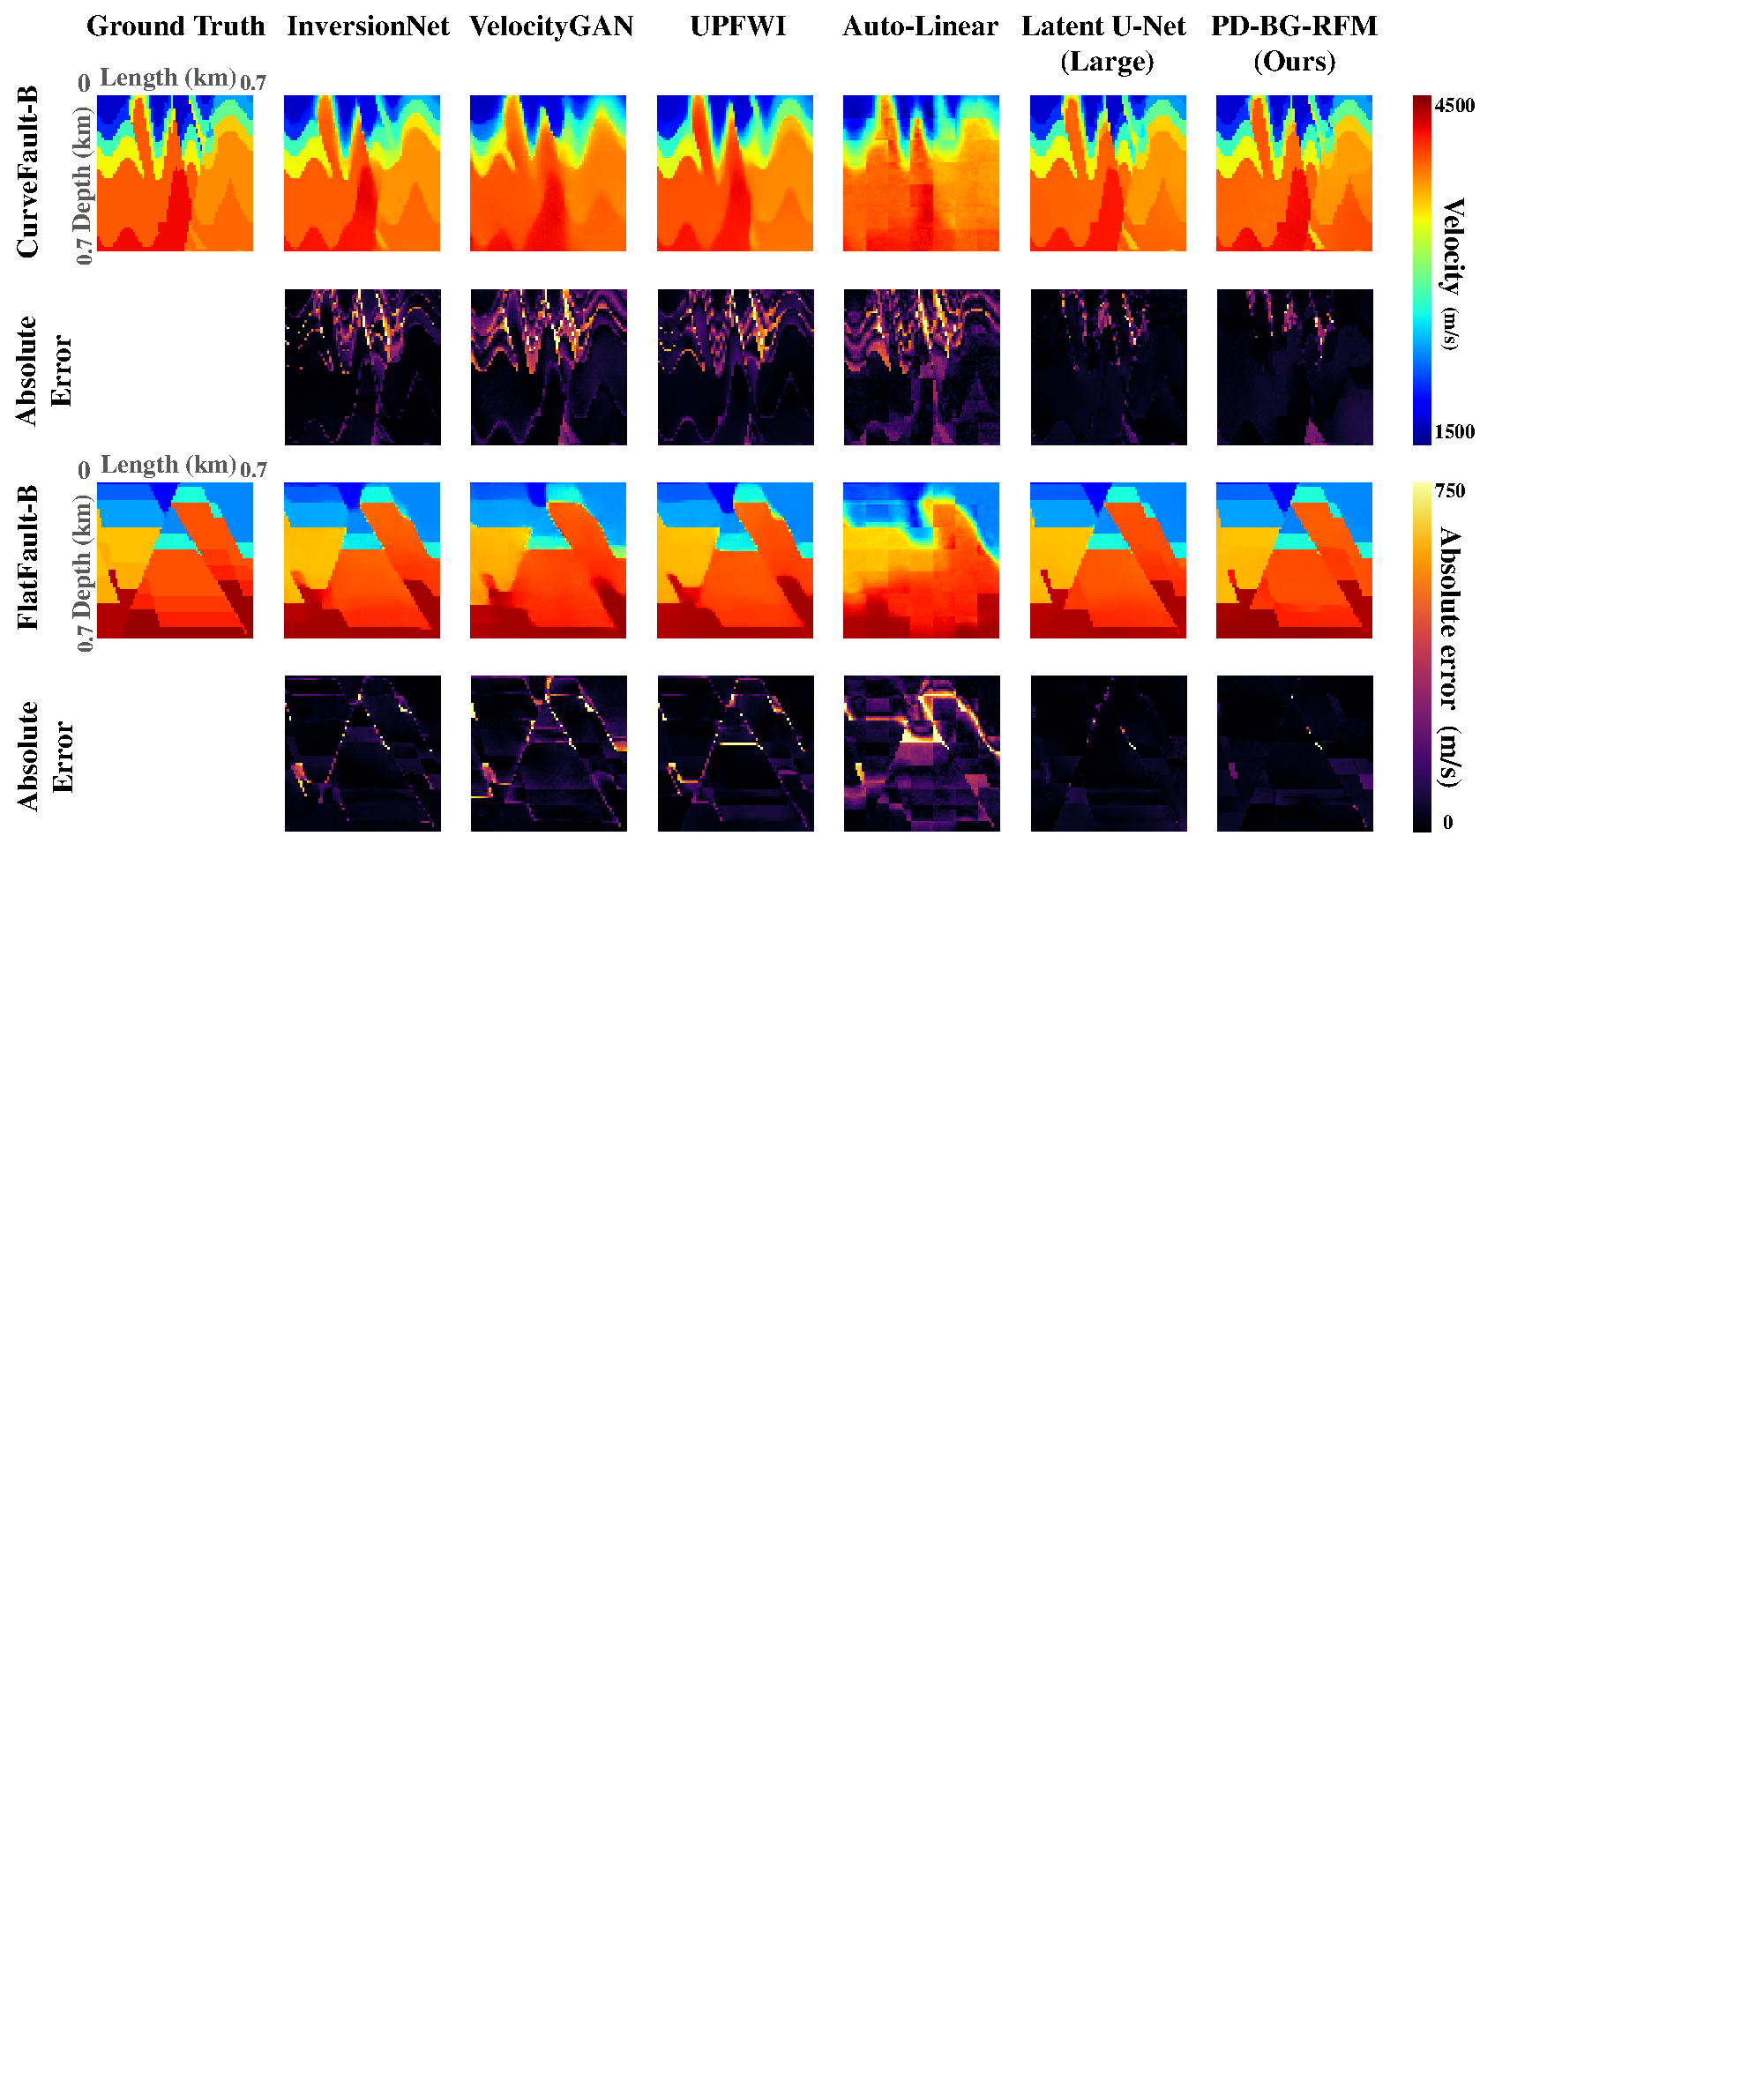
\includegraphics[width=\textwidth]{figures/aaai/qualitative.pdf}
	\caption{Matched-input qualitative results on held-out CurveFault-B and FlatFault-B, highlighting fault and layer-boundary fidelity. Predictions and absolute errors share scales.}
	\label{fig:adapted-qualitative}
\end{figure*}

% BG-REV 2D-H-RESULTS: Rename Experiments to Results; all experiments retained.
\section{Results}

\subsection{Comparison with Existing Methods}
\textbf{Paradigm-level benchmark context.} Table~\ref{tab:main-comparison} contrasts established waveform-based inversion with multimodal constraint integration on OpenFWI, preserving the native observation and evaluation setting of each paradigm. PD-BG-RFM records the strongest value in 21 of 24 subset--metric cells and leads all three metrics on seven of the eight subsets. These results establish multimodal constraint integration as a competitive inversion paradigm across increasingly complex velocity families. Table~\ref{tab:adapted-comparison} then isolates estimator performance under a common multimodal input contract and evaluator. Provenance, scale conversion, parameter counting, and source-protocol details appear in Appendix~\ref{app:benchmark-accounting}.

\begin{table}[t]
		\centering
		\small
		\begin{tabular*}{\columnwidth}{@{\extracolsep{\fill}}l@{\hspace{1.5pt}}c@{\hspace{1.5pt}}c@{\hspace{1.5pt}}c@{\hspace{1.5pt}}c@{\hspace{1.5pt}}c@{\hspace{1.5pt}}c@{}}
			\toprule
			Method & \shortstack{MAE} & \shortstack{RMSE} & \shortstack{SSIM} & \shortstack{$\mathrm{MAE}_L$} & \shortstack{$\mathrm{MAE}_H$} & Params \\
		\midrule
		InversionNet & \underline{0.0149} & 0.0273 & 0.9812 & 0.0180 & \underline{0.0079} & 24.41M \\
		VelocityGAN & 0.0217 & 0.0434 & 0.9727 & 0.0149 & 0.0136 & 25.59M \\
		UPFWI & \textbf{0.0132} & 0.0299 & 0.9895 & \underline{0.0079} & 0.0098 & 19.00M \\
		Auto-Linear & 0.0313 & 0.0593 & 0.9703 & 0.0182 & 0.0229 & 35.47M \\
		\shortstack[l]{Latent U-Net\\(Large)} & 0.0170 & \underline{0.0311} & \underline{0.9910} & \textbf{0.0071} & 0.0134 & 35.12M \\
		\midrule
		\textbf{PD-BG-RFM} & 0.0150 & \textbf{0.0270} & \textbf{0.9913} & 0.0119 & \textbf{0.0065} & \textbf{10.60M} \\
		\bottomrule
		\end{tabular*}
	\caption{Matched-input comparison on 33,600 held-out records. All methods share inputs, split, normalization, and evaluator. Bold and underlined values rank first and second.}
	\label{tab:adapted-comparison}
\end{table}

\textbf{Matched-input estimator comparison.} To complement the paradigm-level comparison, we adapt InversionNet, VelocityGAN, and UPFWI \cite{deng2022openfwi}, Auto-Linear \cite{feng2024autolinear}, and GFI's Latent U-Net (Large) \cite{gupta2025gfi} to the common multimodal input and evaluate all models on identical held-out records with one evaluator. Table~\ref{tab:adapted-comparison} reports their sample-averaged metrics, while Appendix~\ref{app:adapted-accounting} documents implementations and checkpoints. PD-BG-RFM ranks first in RMSE, SSIM, and high-frequency MAE with fewer parameters than every adapted baseline: 10.6M, 44.2\% below the next-smallest model. This efficiency supports asymmetric capacity allocation: deterministic regression handles the background, reserving Flow Matching for the prediction-relative residual characterized by Theorem~1(iii). Figure~\ref{fig:adapted-qualitative} complements these aggregate results with held-out CurveFault-B and FlatFault-B examples. Shared velocity and error scales highlight recovery of faults and layer interfaces while localizing the remaining errors.

\subsection{Condition and Transport Diagnostics}



This section diagnoses two empirical implications of PD-BG-RFM: whether the learned conditions preserve the responsibilities defined by the condition contract and whether prediction-relative residuals satisfy the lower-energy criterion in Theorem~1(iii).
Figure~\ref{fig:condition-contract} tests the representation side of the condition contract. Matched tuples exceed shuffled tuples by median cosine-similarity margins of 0.46 for the background role and 0.35 for the structural role. The fused conditions attain global medians of 0.76 for $\eta_{\mathrm{bg}}$ and 0.66 for $\eta_{\mathrm{str}}$, with cross-role similarity $\chi_{\mathrm{bg,str}}=0.17$. The agreement persists across all eight subsets, providing direct evidence that anchor calibration and role separation survive multimodal fusion.

% BG-REV R1-2C: author-approved new diagnostic interpretation.
\BGRevAdd{The learned routing weights provide a complementary perspective on how the two condition interfaces integrate heterogeneous geophysical observations. Across the 25,222 held-out records containing all four modalities, the background-oriented route assigns its largest average weights to RMS velocity and well logs, whereas the structure-oriented route favors post-stack migrated sections and horizon maps (Figure~\ref{fig:main-role-routing}). These weights are obtained from the trained encoder rather than directly prescribed by the fixed modality-role priors. The observed pattern is consistent with the intended distinction between numerical and structural guidance, while allowing every available modality to contribute to both reconstruction branches.}

% BG-REV FIG-2C: main-text crop of the original appendix figure; original image untouched.
\begin{figure*}[t]
\centering
% BG-REV FIG-2C: pixel-preserving compact crop generated from the original four-panel PNG.
% Only the redundant panel-(d) heading and surrounding whitespace are excluded.
% Appendix B continues to include the byte-identical full diagnostic PNG.
\BGRevFigure{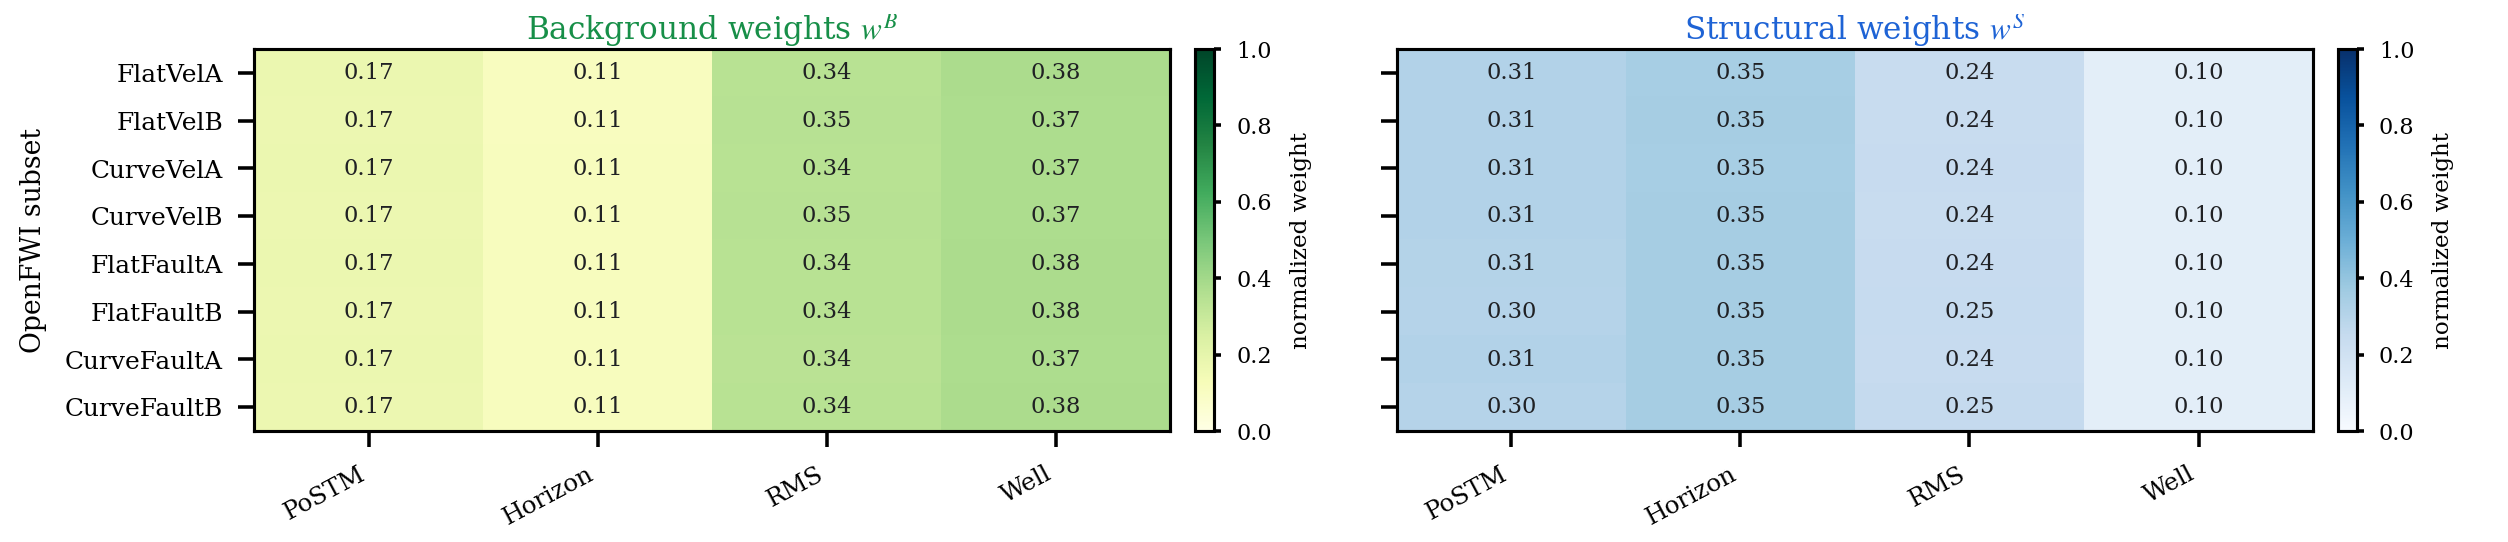
\includegraphics[width=0.93\textwidth]{figures/aaai/role_routing_compact.png}}
\caption{\BGRevAdd{Role-specific reliability routing across the eight OpenFWI subsets. Average normalized weights of the trained background-oriented and structure-oriented interfaces, evaluated on 25,222 held-out records with all four modalities available. The weights are read from the trained encoder, which was regularized using fixed modality-role priors during training. The complete diagnostic figure is provided in Appendix~\ref{app:condition-diagnostics}.}}
\label{fig:main-role-routing}
\end{figure*}

For a field with $d=HW$ pixels, we measure the normalized straight-path target-energy ratio
\begin{equation}
q_T=\frac{d^{-1}\|V-\hat B\|_2^2+1}{d^{-1}\|V\|_2^2+1}.
\label{eq:transport-diagnostic}
\end{equation}
Here $q_T<1$ is equivalent to the condition in Theorem~1(iii).

\begin{figure}[tbp]
		\centering
		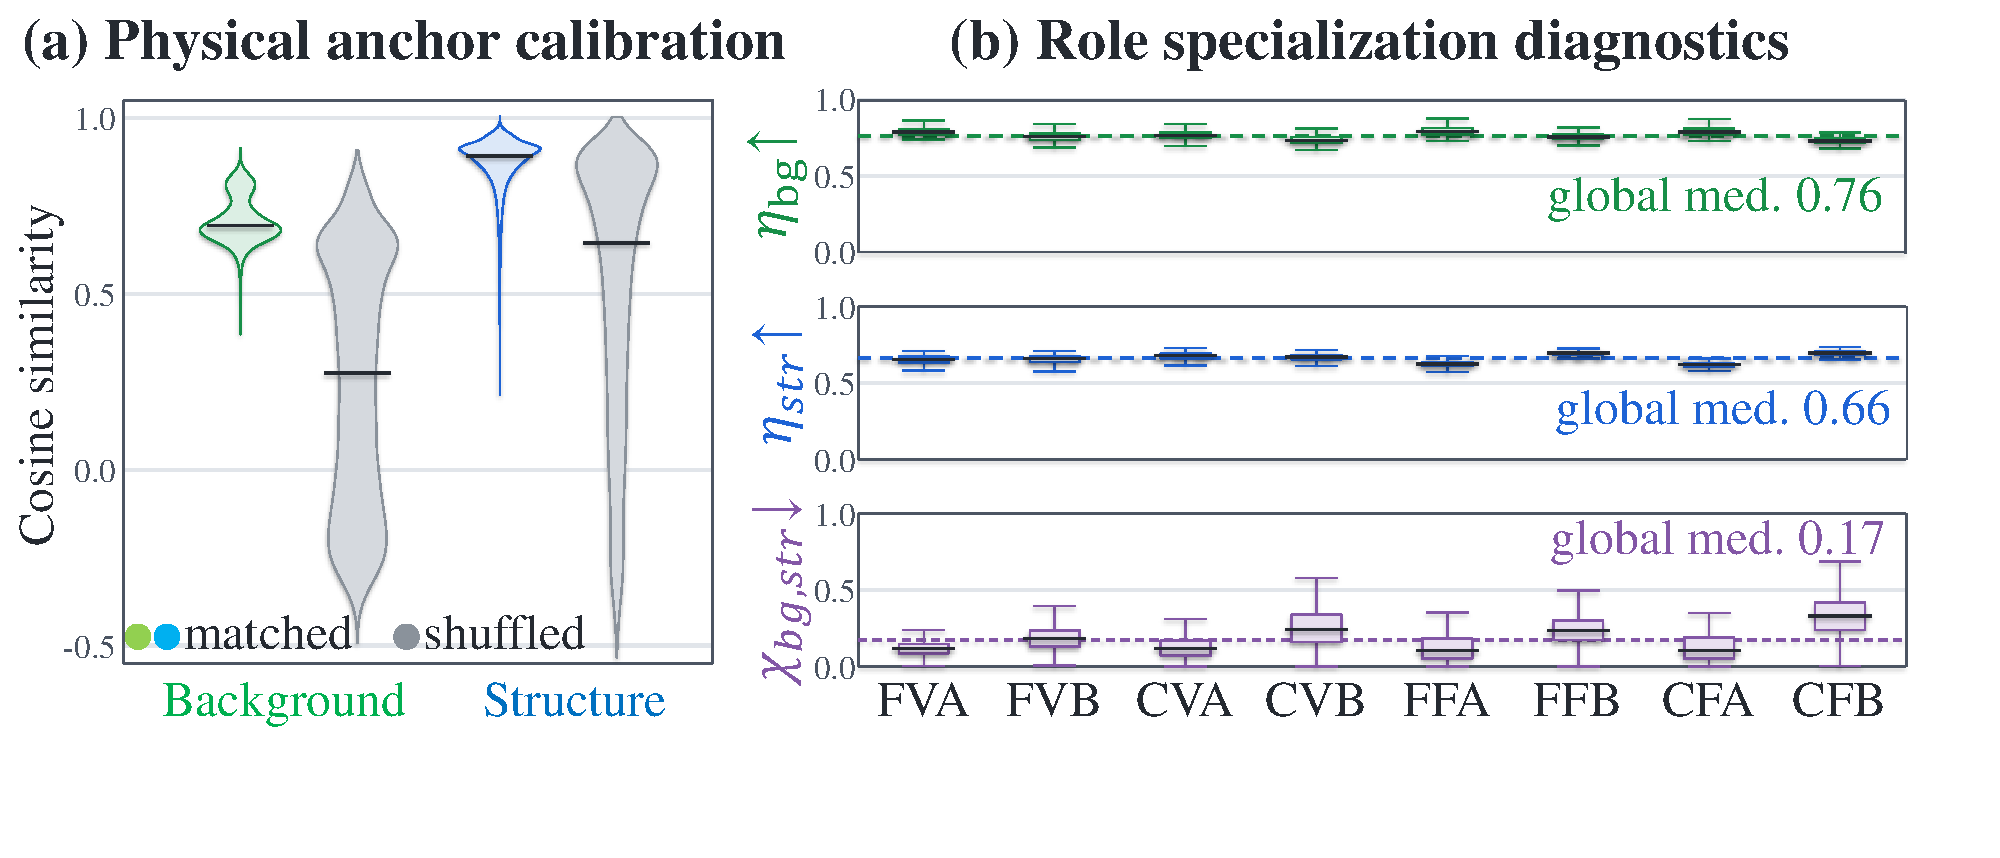
\includegraphics[width=\columnwidth]{figures/aaai/condition_learning.pdf}
	\caption{Condition-routing diagnostics on 33,600 held-out records. (a) Matched--shuffled anchor-similarity margins: 0.46 (background), 0.35 (structural). (b) Role specialization ($\eta_{\mathrm{bg}}$, $\eta_{\mathrm{str}}$) and cross-role similarity ($\chi_{\mathrm{bg,str}}$) by subset. Anchors never enter inference.}
	\label{fig:condition-contract}
\end{figure}

\begin{figure}[tbp]
\centering
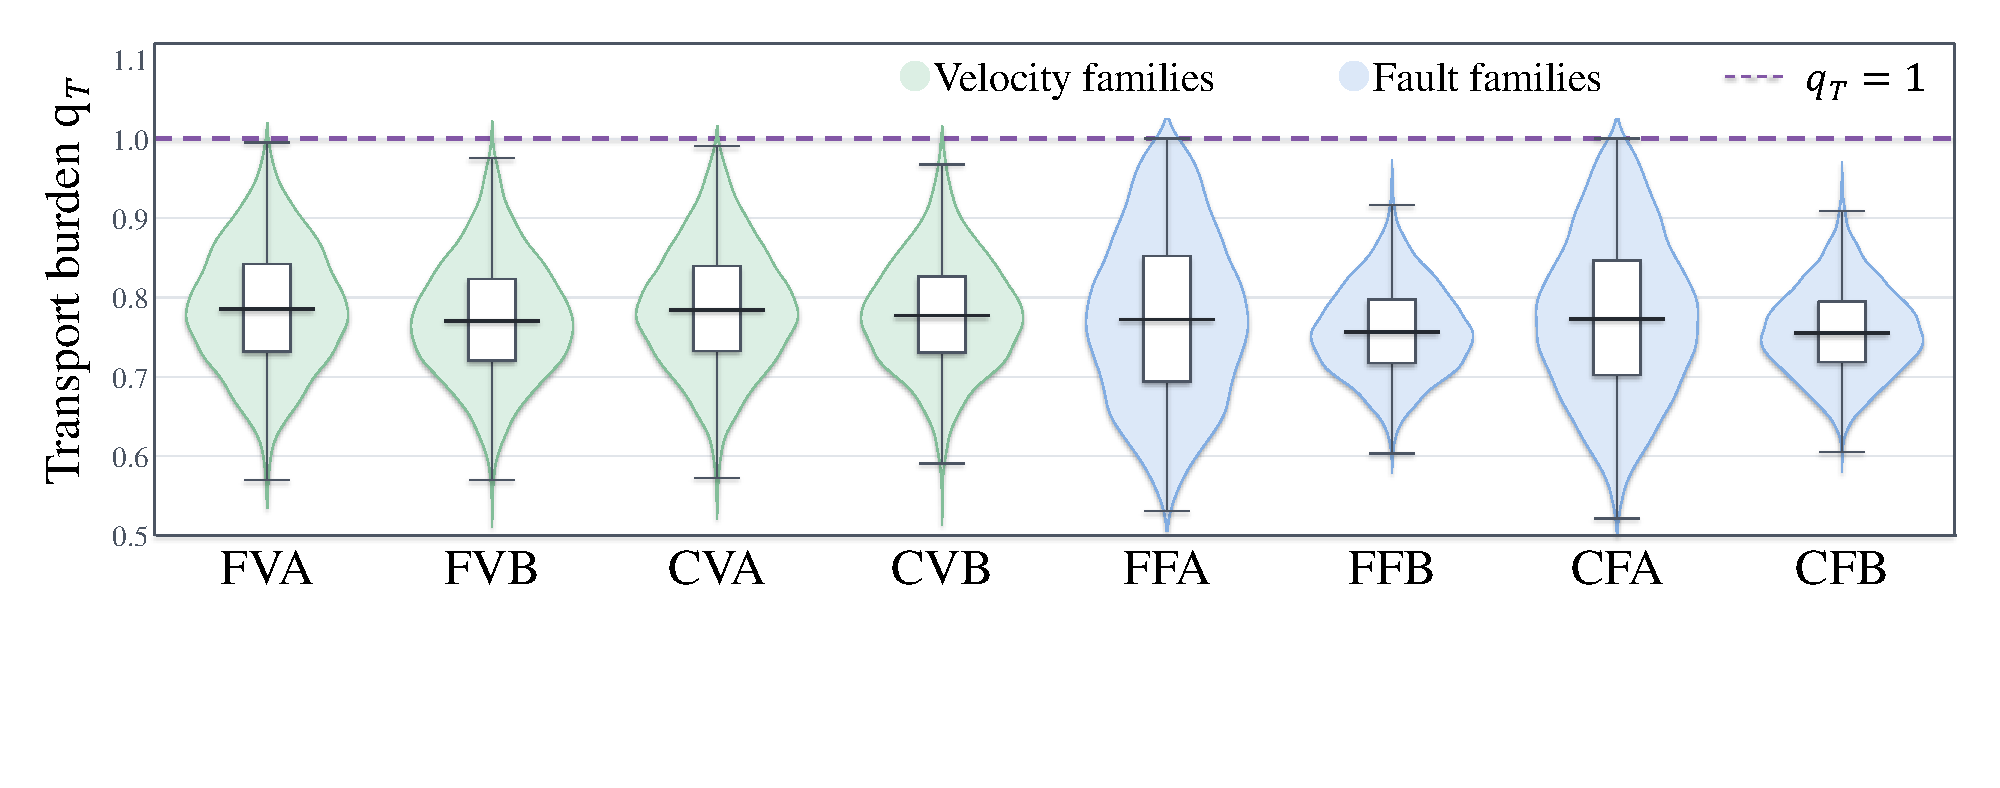
\includegraphics[width=\columnwidth]{figures/aaai/residual_transport.pdf}
\caption{Straight-path target-energy ratio $q_T$ across eight held-out OpenFWI subsets. The dashed line marks $q_T=1$; all 33,600 samples satisfy $q_T<1$.}
\label{fig:residual-transport}
\end{figure}

Figure~\ref{fig:residual-transport} tests this condition on the held-out split. Every one of the 33,600 records satisfies $q_T<1$, with mean 0.772 and bootstrap 95\% confidence interval $[0.771,0.773]$. This corresponds to a 22.8\% average samplewise reduction in normalized straight-path target energy and links the predicted background directly to the intended simplification of residual transport.

Additional condition, background-residual, and missing-modality diagnostics are reported together in Appendix~\ref{app:supplementary-results} under the same held-out protocol.

\subsection{Ablation Study}

Table~\ref{tab:ablation} follows the construction of PD-BG-RFM under a common protocol. Concat-FM uses one fused condition; Decoupled-FM introduces $C_{\mathrm{bg}}$ and $C_{\mathrm{str}}$ but still generates the full field. Uniform Fusion retains the decoupled architecture but removes reliability weighting. The final two variants remove prediction consistency or the background context $\psi_{\mathrm{bg}}(\hat B)$, respectively. Additional controls appear in Appendix~\ref{app:component-ablations}.


% BG-REV 2G-B-P1: Interpret condition separation, complete design, and fusion.
\BGRevAdd{The ablations distinguish the benefit of role-specific conditions from that of organizing the reconstruction around a predicted background. Concat-FM and Decoupled-FM both generate the full velocity field; introducing separate condition interfaces lowers RMSE from 0.0340 to 0.0320 and increases SSIM from 0.9865 to 0.9880, while their high-frequency MAE remains 0.0068. The complete background-and-correction configuration reaches RMSE 0.0270 and the lowest low- and high-frequency MAE among the tested variants. Within this configuration, reliability weighting improves every reported metric over Uniform Fusion, including a reduction in low-frequency MAE from 0.0128 to 0.0119. These comparisons support using role-aware conditions together with an explicit division between deterministic estimation and generative correction, with adaptive fusion regulating the evidence supplied to each role.}

% BG-REV 2G-B-P2: Distinguish prediction consistency from background context.
\BGRevAdd{The reference-related variants further show that the predicted background is useful both as the residual target's origin and as information for the residual generator. Removing prediction consistency raises RMSE to 0.0340 and low-frequency MAE to 0.0156, supporting the use of the same predicted reference for supervision and composition. In the background-context ablation, the deterministic background predictor is retained and its prediction still defines the residual and final sum; only its explicit conditioning input to the residual generator is removed. This variant yields RMSE 0.0410 and high-frequency MAE 0.0100, compared with 0.0270 and 0.0065 for the complete model. Thus, subtracting a background during target construction does not substitute for exposing that background to the learned vector field. Across these controls, the strongest reconstruction combines prediction-relative supervision, background-conditioned correction, and reliability-weighted role interfaces.}

\begin{table}[htbp]
	\centering
	\small
	\begin{tabular*}{\columnwidth}{@{\extracolsep{\fill}}l@{\hspace{2.5pt}}c@{\hspace{2.5pt}}c@{\hspace{2.5pt}}c@{\hspace{2.5pt}}c@{\hspace{2.5pt}}c@{}}
		\toprule
		Variant & MAE $\downarrow$ & RMSE $\downarrow$ & SSIM $\uparrow$ & $\mathrm{MAE}_L\downarrow$ & $\mathrm{MAE}_H\downarrow$ \\
		\midrule
		Concat-FM & 0.0225 & 0.0340 & 0.9865 & 0.0189 & \underline{0.0068} \\
		Decoupled-FM & 0.0205 & 0.0320 & 0.9880 & 0.0175 & \underline{0.0068} \\
		Uniform Fusion & \underline{0.0163} & \underline{0.0290} & \underline{0.9898} & \underline{0.0128} & 0.0072 \\
		\shortstack[l]{w/o Prediction\\Consistency} & 0.0190 & 0.0340 & 0.9875 & 0.0156 & 0.0072 \\
		\shortstack[l]{w/o Background\\Context} & 0.0230 & 0.0410 & 0.9820 & 0.0175 & 0.0100 \\
		\textbf{PD-BG-RFM} & \textbf{0.0150} & \textbf{0.0270} & \textbf{0.9913} & \textbf{0.0119} & \textbf{0.0065} \\
		\bottomrule
	\end{tabular*}
	\caption{Controlled ablations on 33,600 held-out records under shared inputs, split, training budget, evaluator, and 50-step Flow Matching inference. Bold and underlined values rank first and second.}
	\label{tab:ablation}
\end{table}

% BG-REV 2D-H-DISCUSSION: Insert standalone academic Discussion.
\section{Discussion}

% BG-REV 2D-DISC-P1: New Discussion paragraph, colored in review PDF.
\BGRevAdd{The distinction between predicting the velocity background and transporting its remaining variation is not merely a different parameterization of a full-field generator. In PD-BG-RFM, deterministic estimation is assigned the smooth background, while conditional Flow Matching models the correction to that prediction. This allocation makes the two estimation responsibilities explicit: RMS velocity and sparse wells provide information about broad kinematics and absolute scale, while post-stack migrated sections and horizons contribute geometric guidance, without assigning any observation exclusively to either route. The decomposition $V=B+S$ provides an interpretable view of the target, but the transported variable is $V-\hat B$ rather than $S$. It can therefore contain both structure-bearing variation and the correction required by an imperfect background estimate. The distinction allows the two branches to use different estimation mechanisms while contributing to the same depth-domain reconstruction.}

% BG-REV 2D-DISC-P2: New Discussion paragraph, colored in review PDF.
% BG-REV 2G-C-P2: Targeted publication-oriented revision of Discussion paragraph 2.
\BGRevAdd{Prediction consistency gives this allocation a precise operational meaning. The same $\hat B$ defines residual supervision, enters the conditioning of the residual vector field, and is added to the transported endpoint at inference. In the full-field interpretation of Equation~\ref{eq:background-centered-transport}, it also centers the starting distribution on an estimate inferred from the observations, linking the generative reference to the deterministic prediction. As a result, the composed reconstruction error equals the prediction-relative residual error, avoiding a separate background-mismatch term associated with oracle-residual supervision. The residual's low-pass response reflects both background prediction error and detail retained in $\hat B$, so the low-pass matching term supervises the actual residual target. Stop-gradient reuse of the background prediction separates the optimization responsibilities of the branch-exclusive parameters, while the jointly trained condition encoder continues to connect their representations. Thus, the two routes are coupled by a shared numerical reference and jointly learned conditions, with distinct optimization responsibilities.}

% BG-REV 2D-DISC-P3: New Discussion paragraph, colored in review PDF.
% BG-REV 2G-C-P3: Targeted publication-oriented revision of Discussion paragraph 3.
\BGRevAdd{The experiments provide complementary evidence for this reconstruction organization. Under matched multimodal inputs and a shared evaluator, PD-BG-RFM attains the strongest RMSE, SSIM, and high-frequency MAE among the adapted baselines with 10.6M trainable parameters (Table~\ref{tab:adapted-comparison}). The ablations support the combination of role separation, prediction consistency, background context, and reliability weighting that produces these results (Table~\ref{tab:ablation}). The trained condition-routing weights exhibit a corresponding division of emphasis: RMS velocity and well logs receive the largest average background-oriented contributions, whereas migrated sections and horizons contribute most strongly to the structure-oriented route on complete-modality records. Learned under role-specific reliability priors, this pattern accords with the intended distinction between numerical and geometric guidance. The straight-path diagnostic adds a target-level counterpart: prediction-relative residuals satisfy the lower-energy criterion of Theorem~1(iii) across the evaluated held-out records (Figure~\ref{fig:residual-transport}). Together, reconstruction metrics, routing behavior, and target-energy measurements support a common organization in which the predicted background provides the reference for a structurally guided correction.}

% BG-REV 2D-DISC-P4: New Discussion paragraph, colored in review PDF.
% BG-REV 2G-C-P4: Targeted publication-oriented revision of Discussion paragraph 4.
\BGRevAdd{These findings concern depth-domain velocity reconstruction from precomputed and interpreted geophysical constraints in synthetic OpenFWI-derived settings. RMS velocity and post-stack migrated images supply processed kinematic and imaging information, while horizon masks and sparse well-velocity columns provide idealized structural and local calibration inputs; raw shot gathers are not supplied to the inversion network at inference. Within this setting, deterministic background prediction and residual transport address complementary aspects of model building: establishing broad velocity levels and refining the structure relative to those levels. The synthetic horizon masks and sampled well columns are derived from reference velocity models, defining the structural and local-control information available in the evaluation. The geophysical value of the formulation is therefore its explicit connection between numerical velocity guidance and interface geometry in a common depth-domain estimate. This offers a methodological basis for using processed observations and interpretation products together, with their respective reconstruction roles made explicit.}

% BG-REV 2D-H-CONCLUSIONS: Rename Conclusion to Conclusions; original paragraph preserved.
\section{Conclusions}
% BG-REV 2H-CONCLUSIONS: Complete replacement paragraph, blue in author-review PDF.
\BGRevAdd{We introduced Physics-Decoupled Background-Guided Residual Flow Matching (PD-BG-RFM) for velocity reconstruction from processed seismic and interpreted geophysical constraints. The method organizes velocity estimation into two complementary responsibilities: role-aware multimodal conditions guide direct background prediction, while conditional Flow Matching models the correction relative to that prediction. By reusing the same background estimate for residual supervision, vector-field conditioning, and final composition, the formulation establishes a prediction-consistent connection between the two routes. In full-field coordinates, this connection corresponds to transport from an observation-dependent reference centered on the predicted background. The composition and low-pass identities characterize the resulting correction, and the straight-path criterion identifies when its target energy is reduced. Matched-input experiments across held-out OpenFWI-derived samples achieve the best RMSE, SSIM, and high-frequency MAE among the evaluated adapted baselines with 10.6 million parameters; ablations and routing diagnostics provide complementary evidence for the proposed organization. The central insight is that a predicted background can serve as the common numerical reference connecting heterogeneous geophysical guidance and generative structural correction.}

\bibliography{references}

\ifaaaiwithappendix
\clearpage
\setcounter{secnumdepth}{1}
\appendixtitles{yes}
\appendixstart
\appendix
% Prefix appendix equations, figures, and tables with their lettered section.
\numberwithin{equation}{section}
\numberwithin{figure}{section}
\numberwithin{table}{section}
\section{Theoretical Derivations and Proofs}
\label{app:residual-proofs}
This appendix proves Theorem~1 under its stated assumptions and derives the objective implications summarized by Corollary~1.

\subsection{Proof of Theorem~1}
\paragraph{(i) Composition consistency.}
Let $R_{\hat B}=V-\hat B$ and $\hat V=\hat B+\hat R$. Then
\begin{equation}
\hat V-V=\hat B+\hat R-V=\hat R-(V-\hat B)=\hat R-R_{\hat B}.
\end{equation}
For $R_B=V-B$, adding and subtracting $B$ instead gives
\begin{equation}
\hat V-V=(\hat B-B)+(\hat R-R_B).
\end{equation}
Thus even a perfect oracle-residual prediction leaves the composition error $\hat B-B$, whereas a perfect prediction-consistent residual reconstructs $V$ exactly. This proves Theorem~1(i).

\paragraph{(ii) Low-pass burden identity.}
Let $P_L$ be linear, define $P_H=I-P_L$, and set $B=P_L(V)$. Then
\begin{align}
P_L(V-\hat B)
&=P_L(V)-P_L(\hat B)\\
&=B-\bigl(\hat B-P_H(\hat B)\bigr)\\
&=(B-\hat B)+P_H(\hat B).
\end{align}
This proves Theorem~1(ii). The proof does not assume that $P_L$ is idempotent. In particular, belonging to $\operatorname{Range}(P_L)$ would not imply $P_L(\hat B)=\hat B$ for the stride-one average pool used here. Because the two terms may cancel, the equality is not an additive decomposition of their norms.

\paragraph{(iii) Straight-path transport energy.}
Let $C=(C_{\mathrm{str}},\hat B)$ and assume the conditional densities exist. For fixed $C$, the transform $T_{\hat B}(v)=v-\hat B$ has inverse $T_{\hat B}^{-1}(r)=r+\hat B$ and Jacobian determinant one. The change-of-variables formula gives
\begin{equation}
p_{R_{\hat B}}(r\mid C)=p_V(r+\hat B\mid C).
\end{equation}
Translation invariance of differential entropy then yields $h(R_{\hat B}\mid C)=h(V\mid C)$ whenever these entropies are finite. The accompanying energy comparison evaluates the Flow Matching target induced by the routed residual.

Now let $\xi\sim\mathcal N(0,I_d)$ be independent of $(V,C_{\mathrm{str}},\hat B)$, and define $u_V=V-\xi$ and $u_R=(V-\hat B)-\xi$. Independence and $\mathbb E[\xi]=0$ give
\begin{align}
\mathbb E\|u_R\|^2
&=
\mathbb E\|V-\hat B\|^2+d,\\
\mathbb E\|u_V\|^2
&=
\mathbb E\|V\|^2+d.
\end{align}
Subtracting proves Eq.~\ref{eq:transport-condition}. For a fixed sample $(V,\hat B)$, taking expectation only over $\xi$ gives
\begin{equation}
\frac{\mathbb E_{\xi}[d^{-1}\|u_R\|^2\mid V,\hat B]}
{\mathbb E_{\xi}[d^{-1}\|u_V\|^2\mid V,\hat B]}
=
\frac{d^{-1}\|V-\hat B\|^2+1}{d^{-1}\|V\|^2+1}.
\end{equation}
This is exactly the sample-level diagnostic $q_T$. A value below one verifies the corresponding samplewise energy condition in the stated normalized coordinates, and its held-out distribution summarizes the routing effect across the test set. This proves Theorem~1(iii).

\subsection{Derivation of Corollary~1}
Equation~\ref{eq:composition-consistent} selects the prediction-relative reference used by residual supervision and final composition, while Eq.~\ref{eq:low-frequency-burden} determines the matching target in the low-pass residual term. Together with the conditional factorization in Definition~1, these identities yield the objective construction summarized by Corollary~1 and instantiated in Eqs.~\ref{eq:background-loss}, \ref{eq:residual-loss}, and~\ref{eq:gradient-contract}. Equation~\ref{eq:transport-condition} supplies the post-training diagnostic $q_T$.


\section{Supplementary Results and Diagnostics}
\label{app:supplementary-results}

\subsection{Data-Level Motivation Analysis}
Figure~\ref{fig:motivation} uses a training-only analysis to quantify the degree-of-freedom asymmetry that motivates the condition contract. From each of the eight OpenFWI training subsets, we select 1,000 records with analysis seed 2027 after fixing the global split with seed 42. The decomposition uses the same stride-one $5\times5$ average-pooling operator as the method and satisfies $V=B+S$ to a maximum numerical error of $1.11\times10^{-16}$. No model, checkpoint, or learned dimensionality reducer enters this analysis.

Let $\{\lambda_j\}$ be the nonzero eigenvalues of a component's sample covariance. We summarize its effective degrees of freedom by the participation-ratio rank
\begin{equation}
r_{\mathrm{eff}}=\frac{\left(\sum_j\lambda_j\right)^2}{\sum_j\lambda_j^2}.
\label{eq:effective-rank}
\end{equation}
Table~\ref{tab:effective-rank} resolves the aggregate curves in Figure~\ref{fig:motivation} by subset. The structural complement has higher effective rank in all eight velocity families, from a $12.0\times$ gap on FlatVel-A to a $38.7\times$ gap on CurveFault-B. Across subsets, the median ranks are 4.95 for the background and 54.03 for the structural complement. This consistent separation supplies a data-level basis for assigning the concentrated background to deterministic prediction and the higher-dimensional correction to generative transport.

\begin{table}[H]
\centering
\small
\begin{tabular}{@{}lrr@{}}
\toprule
OpenFWI subset & Background $B$ & Structure $S$ \\
\midrule
FlatVel-A & 2.02 & 24.26 \\
FlatVel-B & 5.66 & 39.67 \\
CurveVel-A & 2.59 & 58.52 \\
CurveVel-B & 7.53 & 200.89 \\
FlatFault-A & 3.06 & 37.83 \\
FlatFault-B & 7.54 & 289.69 \\
CurveFault-A & 4.24 & 49.54 \\
CurveFault-B & 10.54 & 407.91 \\
\midrule
Median & 4.95 & 54.03 \\
\bottomrule
\end{tabular}
\caption{Participation-ratio effective rank of the background and structural complement on 1,000 fixed training records per OpenFWI subset.}
\label{tab:effective-rank}
\end{table}

\subsection{Extended Qualitative Comparisons}
The following panels extend the matched-input comparison with one fixed-rule representative from each OpenFWI subset. The cases are selected from the same globally held-out manifest as Table~\ref{tab:adapted-comparison}; the deterministic selection protocol is described in Appendix~\ref{app:adapted-accounting}.

\begin{figure*}[p]
\centering
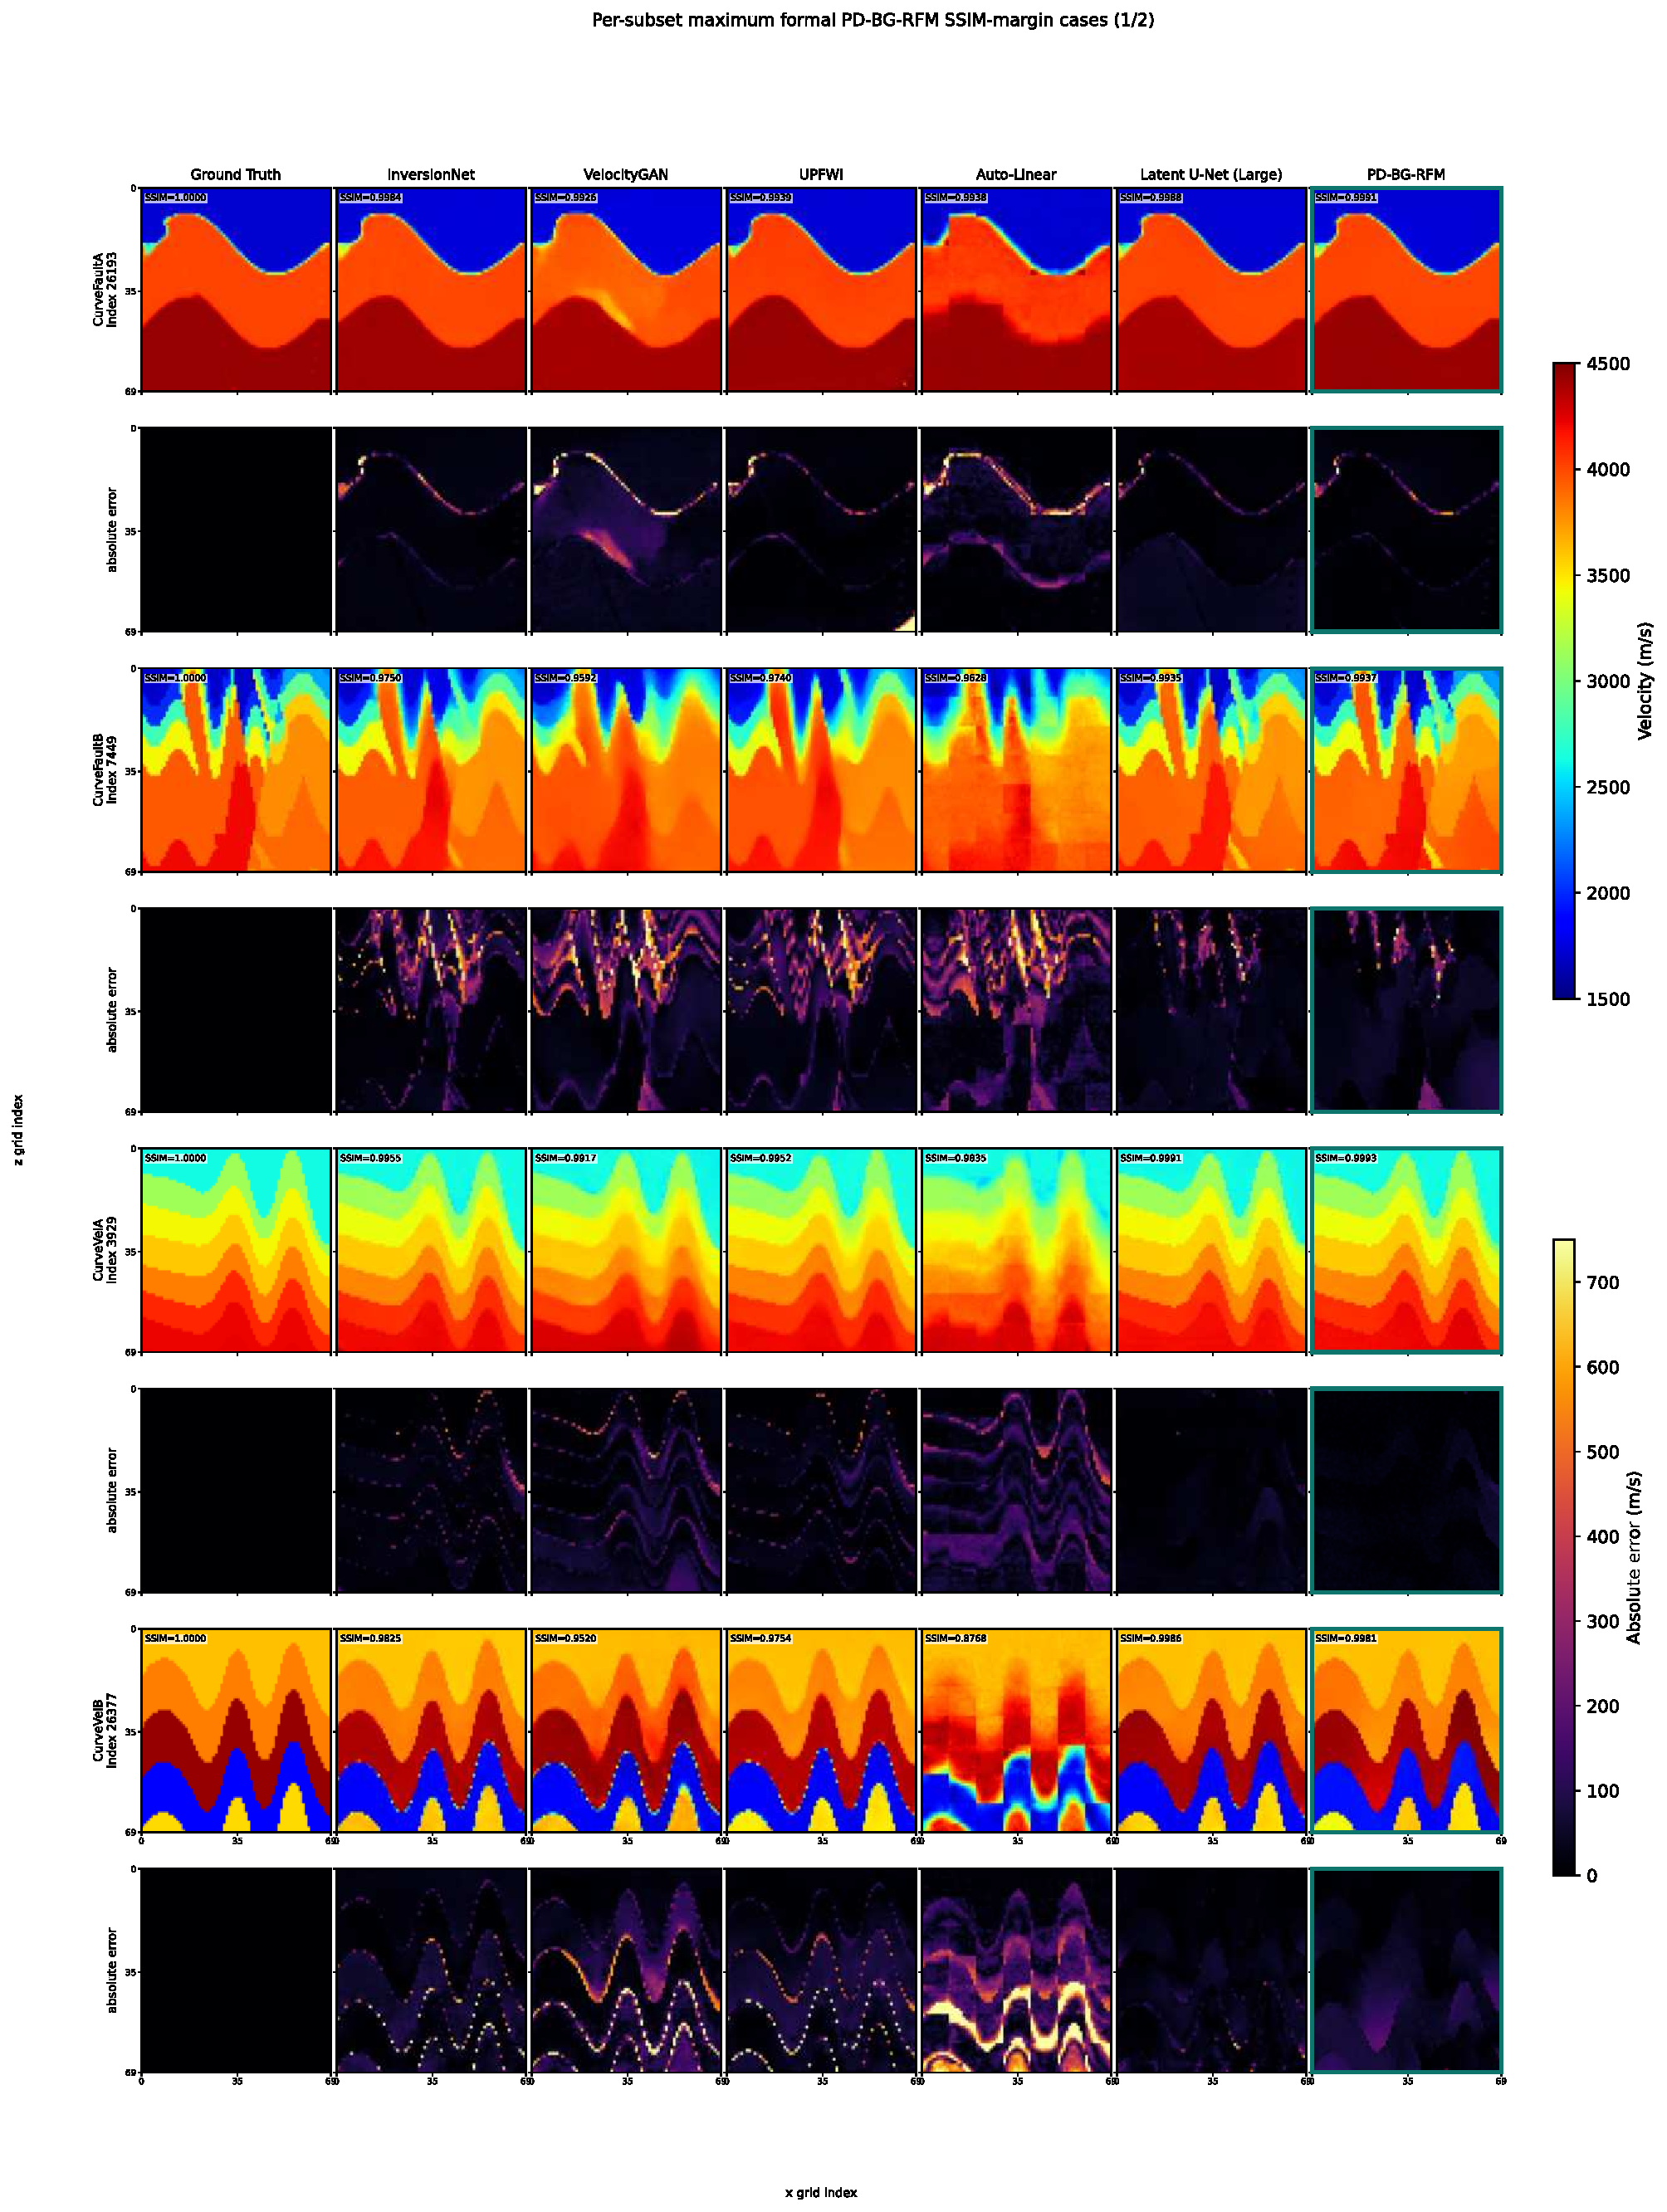
\includegraphics[width=\textwidth,height=0.82\textheight,keepaspectratio]{figures/aaai/table2_representative_cases_1.pdf}
\caption{Fixed-rule qualitative cases for the first four OpenFWI subsets, selected by maximum formal SSIM margin. Display conventions follow Figure~\ref{fig:adapted-qualitative}.}
\label{fig:table2-representative-a}
\end{figure*}

\begin{figure*}[p]
\centering
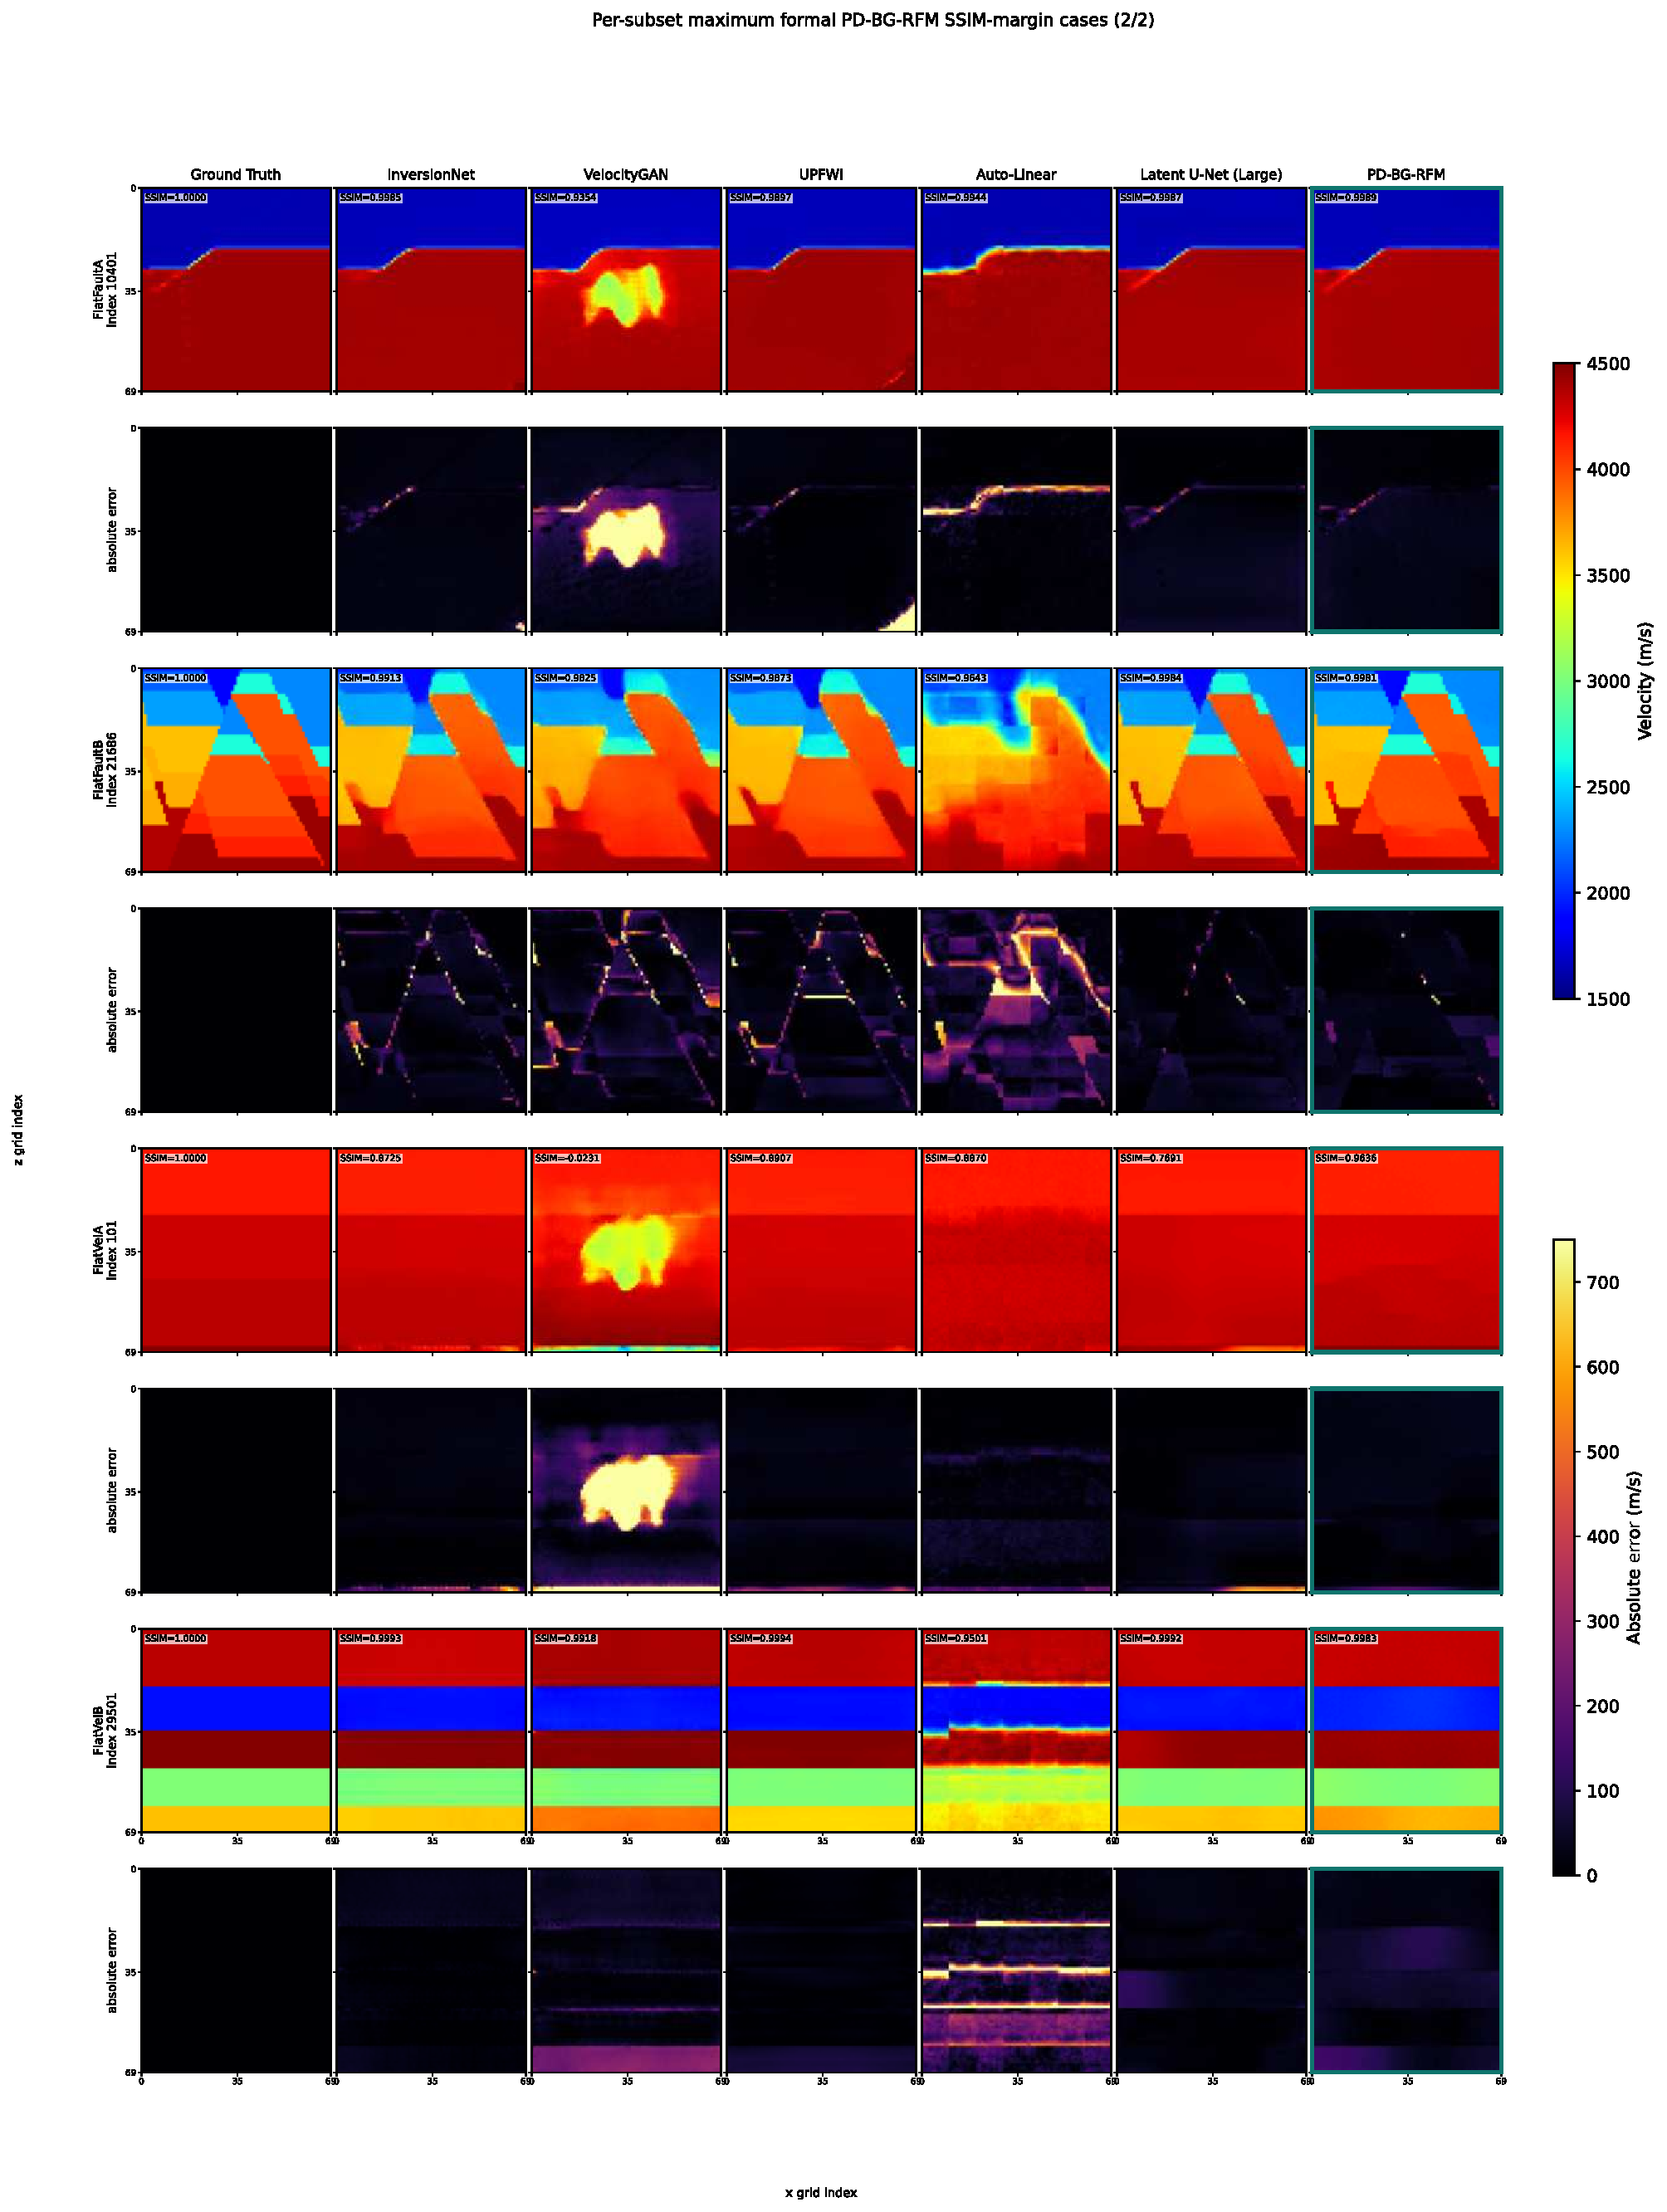
\includegraphics[width=\textwidth,height=0.82\textheight,keepaspectratio]{figures/aaai/table2_representative_cases_2.pdf}
\caption{Fixed-rule qualitative cases for the remaining four OpenFWI subsets under the selection and display conventions of Figure~\ref{fig:table2-representative-a}.}
\label{fig:table2-representative-b}
\end{figure*}

\begin{figure*}[p]
\centering
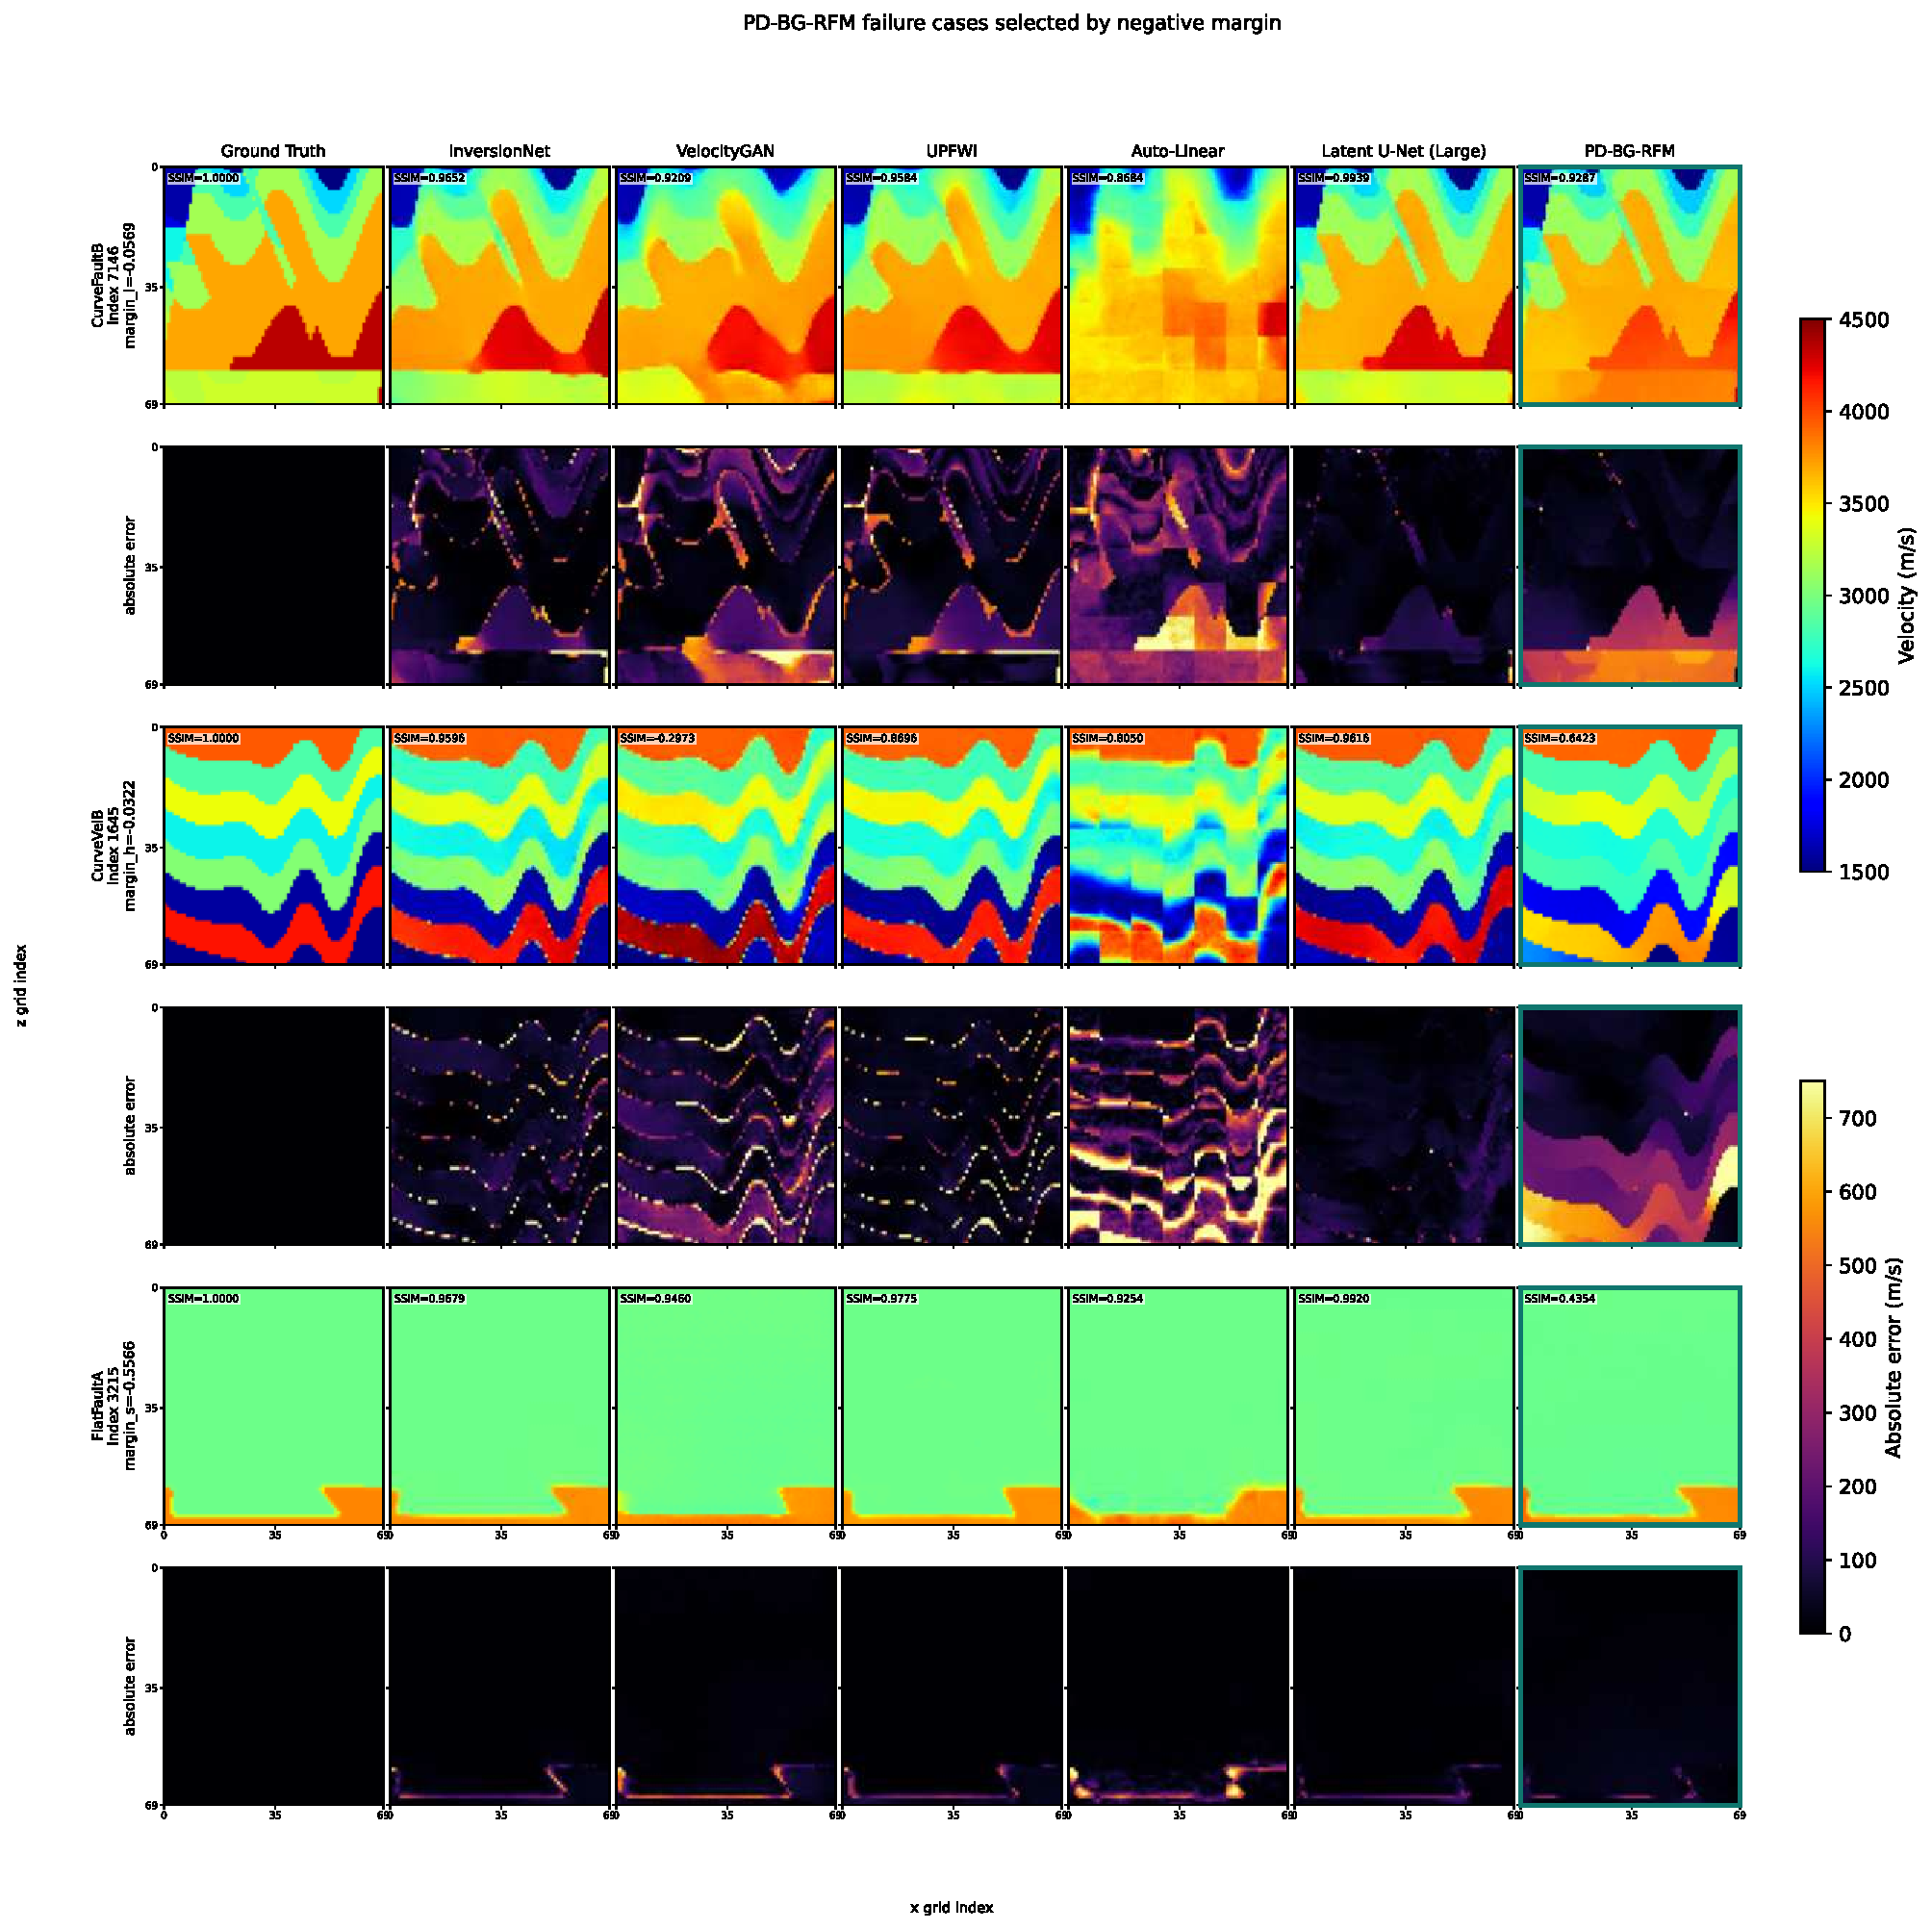
\includegraphics[width=0.99\textwidth]{figures/aaai/table2_failure_cases.pdf}
\caption{Fixed-rule failure cases with the most negative low-frequency, high-frequency, and SSIM margins, respectively.}
\label{fig:table2-failures}
\end{figure*}

\subsection{Additional Component Ablations}
\label{app:component-ablations}
The core attribution table isolates the construction sequence from condition decomposition to background residualization and prediction consistency. The following controls test complementary components without obscuring that chain.
\begin{table}[t]
\centering
\small
\begin{tabular}{@{}p{0.31\columnwidth}@{\hspace{4pt}}p{0.57\columnwidth}@{}}
\toprule
Variant & Isolated factor \\
\midrule
w/o background context & Removes $\psi_{\mathrm{bg}}(\hat B)$ from residual FM. \\
Direct residual predictor & Replaces FM with deterministic residual regression. \\
Uniform fusion & Replaces Eq.~\ref{eq:reliability-fusion} by equal weights over available inputs. \\
w/o condition objective & Sets $\lambda_C=0$ while preserving the routing architecture. \\
\bottomrule
\end{tabular}
\caption{Definitions of additional component controls. They use the data, evaluator, and validation-based checkpoint selection of the core ablations.}
\label{tab:component-ablations}
\end{table}

\subsection{Condition and Transport Diagnostics}
\subsubsection{Condition contract.}
\label{app:condition-diagnostics}
For a feature map $C$, define $M_L(C)=\operatorname{mean}|P_L(C)|$ and $M_H(C)=\operatorname{mean}|P_H(C)|$. The fused-feature diagnostic reports
\begin{align}
\eta_{\mathrm{bg}}&=\frac{M_L(C_{\mathrm{bg}})}{\max(M_L(C_{\mathrm{bg}})+M_H(C_{\mathrm{bg}}),\epsilon)},\\
\eta_{\mathrm{str}}&=\frac{M_H(C_{\mathrm{str}})}{\max(M_L(C_{\mathrm{str}})+M_H(C_{\mathrm{str}}),\epsilon)}.
\end{align}
Larger values indicate stronger agreement with the intended frequency role. Together with separate per-modality squared-energy ratios, anchor alignment, pairwise retrieval, and learned reliability routing, these diagnostics characterize the condition contract from complementary views.

Figure~\ref{fig:full-condition-diagnostics} expands the main-text condition analysis. Pairwise retrieval measures cross-modal specificity within each role, while the anchor distributions reproduce the strict matched--deranged test over all held-out records. The learned routing weights provide the most direct audit of the block-triangular interfaces: RMS velocity and wells receive the largest background weights, whereas PoSTM and horizons receive the largest structural weights. These weights are read from the encoder's forward routing outputs rather than copied from the fixed reliability priors. Routing averages use the 25,222 held-out records containing all four modalities; unavailable modalities otherwise receive zero weight and the available weights remain normalized.

\begin{figure*}[t]
\centering
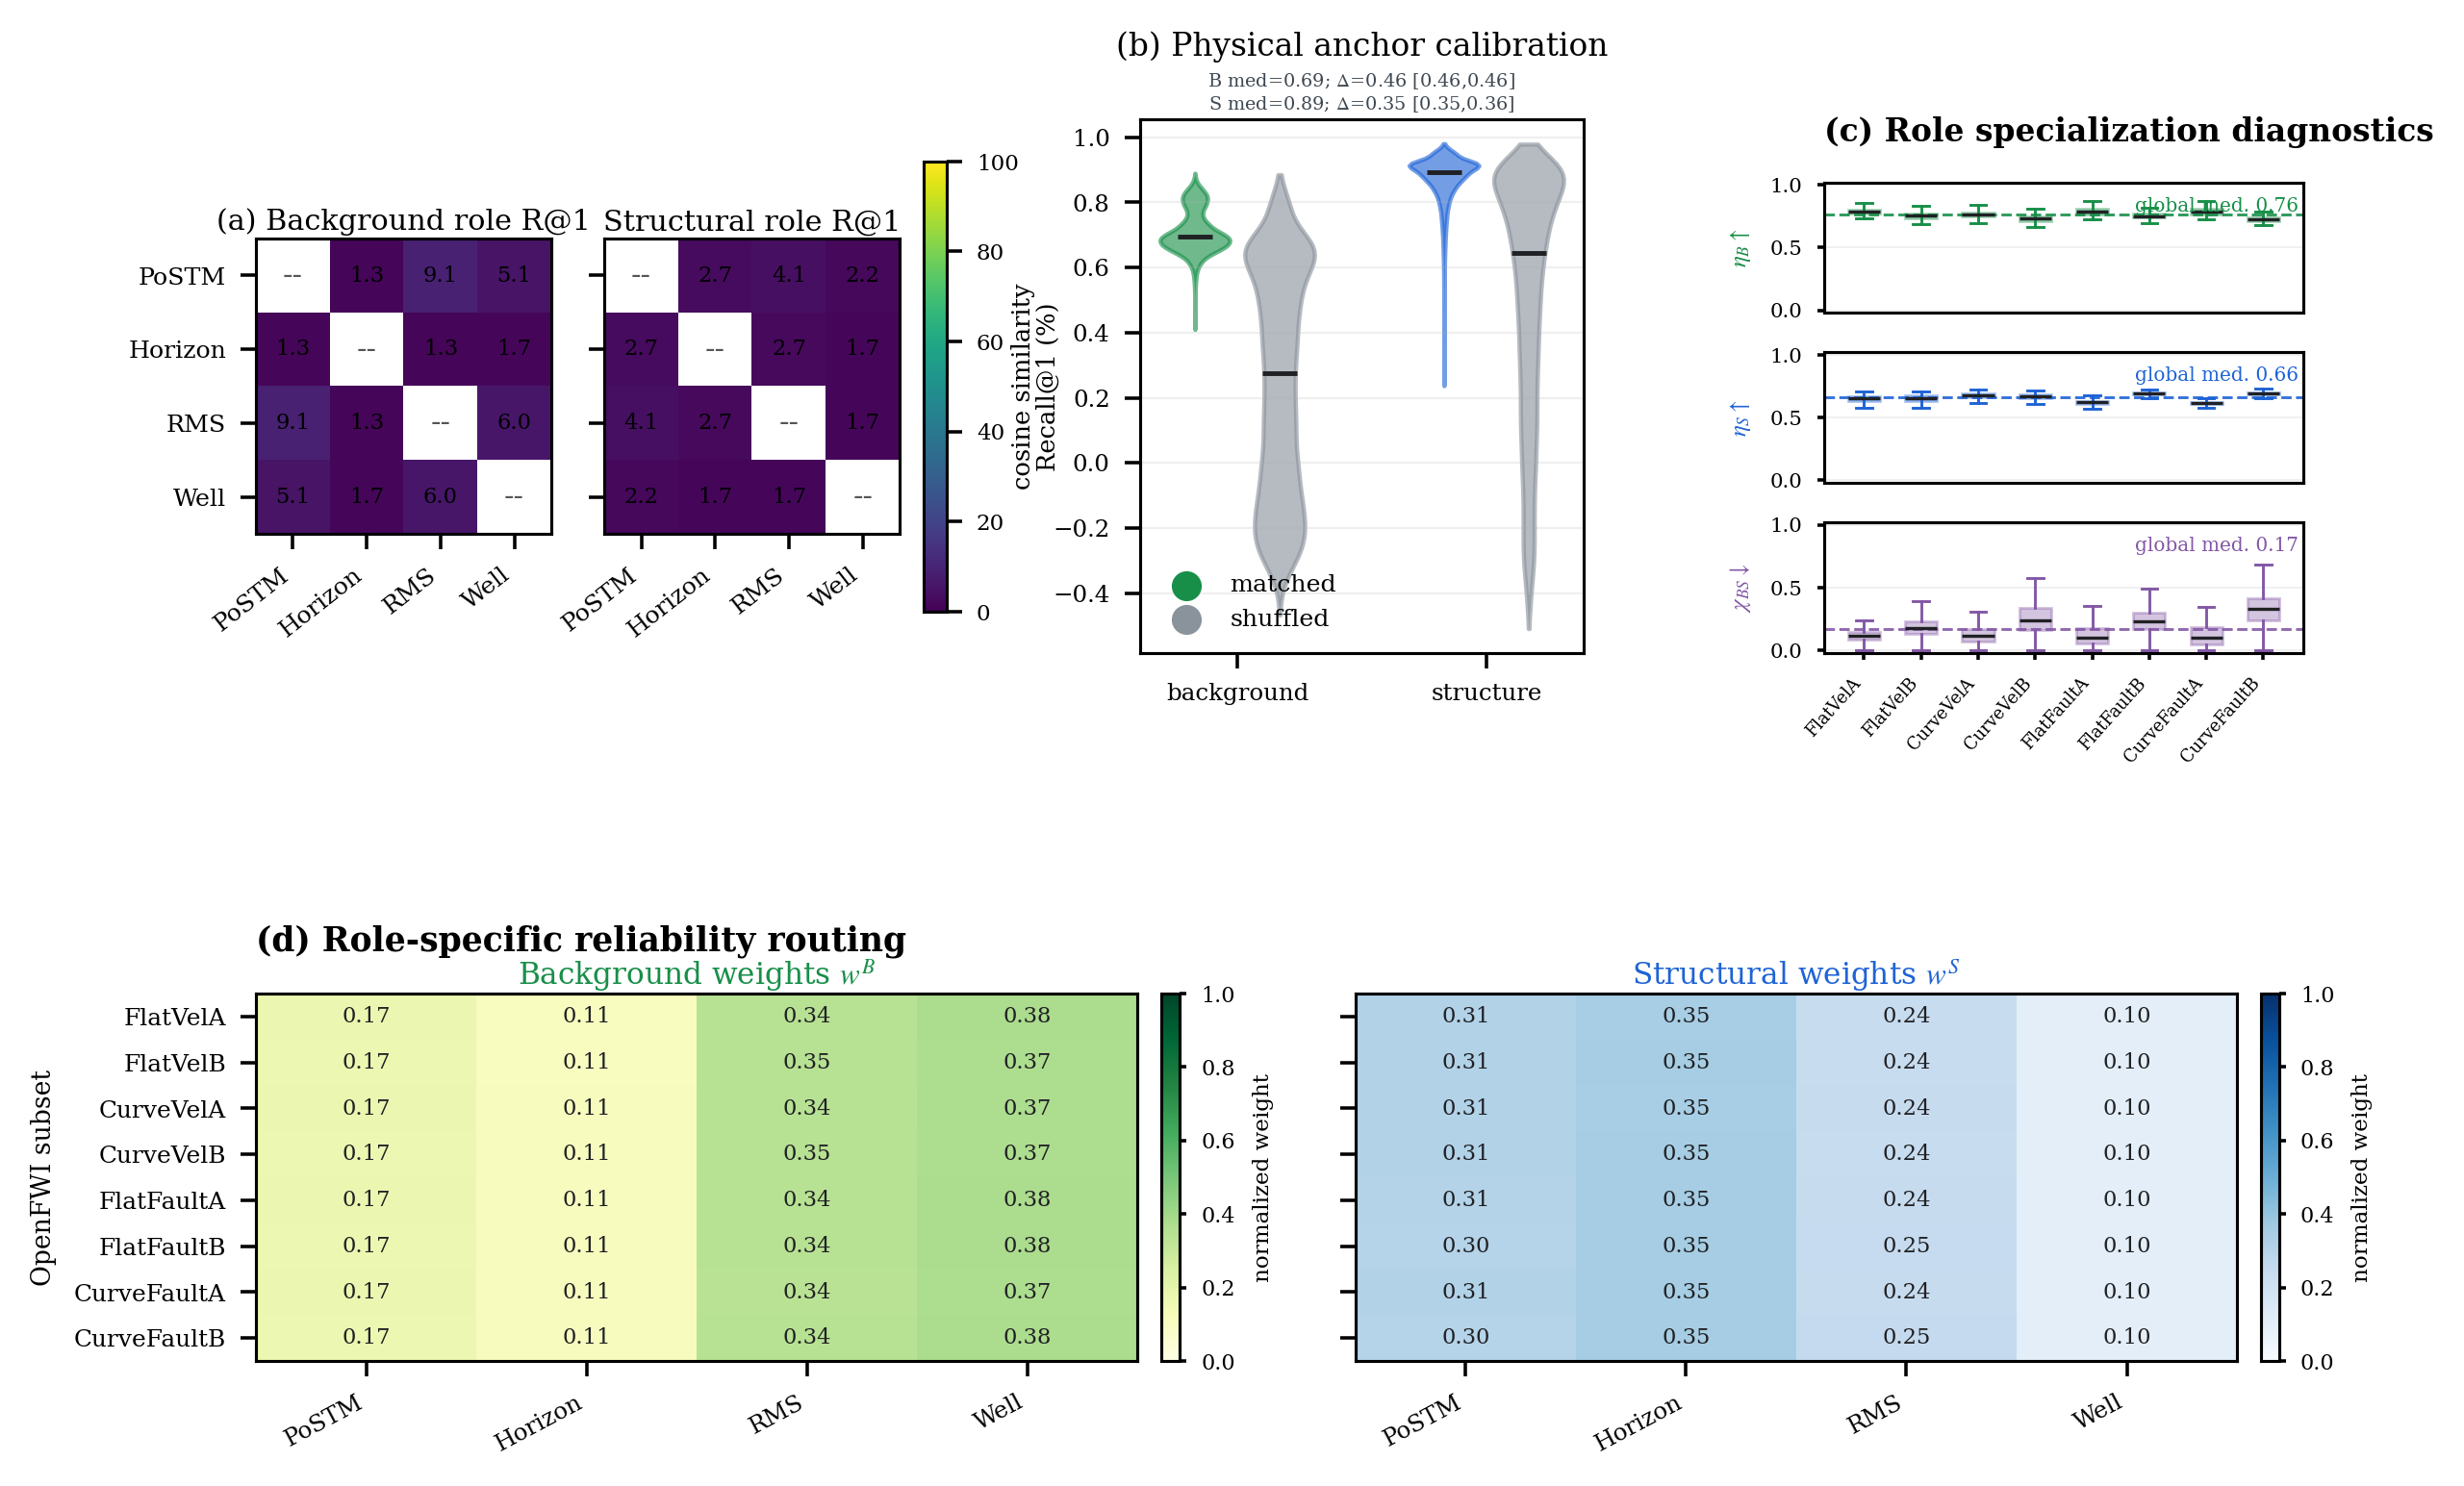
\includegraphics[width=0.98\textwidth]{figures/aaai/appendix_full_condition_diagnostics.png}
\caption{Full condition-contract diagnostics. (a) Cross-modal retrieval-at-one matrices for background and structural role projections; same-modality entries are omitted. (b) Matched and strictly deranged similarities to the training-only physical anchors on 33,600 held-out records. (c) Role-specialization and cross-role-similarity distributions by subset. (d) Learned role-specific routing weights averaged over 25,222 complete-modality held-out records.}
\label{fig:full-condition-diagnostics}
\end{figure*}

\subsubsection{Background-residual transport.}
\label{app:background-diagnostics}
The implementation retains the artifact key \texttt{rho\_B} for backward compatibility, but the paper denotes it by $\rho_{L/H}$. With $d=HW$, the two residual-burden diagnostics are
\begin{align}
\rho_{L/H}
&=\frac{\operatorname{mean}|P_L(V-\hat B)|}
{\operatorname{mean}|P_H(V)|+10^{-6}},\\
e_{R/V}
&=\frac{d^{-1}\|V-\hat B\|_2^2}
{d^{-1}\|V\|_2^2+10^{-8}}.
\end{align}
The first normalizes residual low-pass magnitude by complementary target-detail magnitude, whereas the second measures residual-to-full-field squared energy. We additionally report background MAE, $\epsilon_H^B=\operatorname{mean}|P_H(\hat B)|$, and $q_T$ from Eq.~\ref{eq:transport-diagnostic}. Theorem~1(ii) explains the numerator of $\rho_{L/H}$, while Theorem~1(iii) gives the exact interpretation of $q_T$. These are diagnostics, not training-time gates.

\subsection{Missing-Modality Robustness}
\label{app:missing-modality}
We evaluate a fixed checkpoint with full input, each principal modality removed, both well log and RMS velocity removed, and PoSTM alone. In the target acquisition setting, RMS velocity is part of the standard available observation contract and is assumed to be available at deployment. Thus, the RMS-missing rows are stress tests for observation-coverage robustness rather than standard operating scenarios; their sharp degradation is consistent with RMS velocity carrying the smooth background scale. No retraining or test-time adaptation is performed. Absolute metrics measure retained accuracy, while changes from full input quantify degradation as evidence is removed. Reliability weighting is evaluated as an adaptive fusion mechanism rather than a robustness guarantee. These subsets distinguish the loss of sparse calibration from well logs, interpreted structure from horizons, smooth kinematics from RMS velocity, and all auxiliary magnitude-calibrating evidence. PoSTM alone provides the most severe setting and measures how much reconstruction quality remains under structural imaging only.

\begin{table}[t]
\centering
\small
\begin{tabular}{@{}l@{\hspace{8pt}}c@{\hspace{8pt}}c@{\hspace{8pt}}c@{}}
\toprule
Observation subset & MAE & RMSE & SSIM \\
\midrule
Full input & 0.0150 & 0.0269 & 0.9915 \\
w/o well-log & 0.0168 & 0.0295 & 0.9899 \\
w/o horizon & 0.1011 & 0.1669 & 0.8202 \\
w/o RMS velocity & 0.3947 & 0.4705 & 0.0753 \\
w/o well-log + RMS velocity & 0.4684 & 0.5303 & 0.0192 \\
PoSTM only & 0.4706 & 0.5356 & 0.0154 \\
\bottomrule
\end{tabular}
\caption{Missing-modality evaluation of a fixed PD-BG-RFM checkpoint without retraining or test-time adaptation.}
\label{tab:missing-modality}
\end{table}

\section{Complete Condition-Learning Objective}
\label{app:condition-objective}
\subsection{Reliability-Weighted Fusion}
Restoring the sample index suppressed in Eq.~\ref{eq:reliability-fusion}, let $a_{i,m}\in\{0,1\}$ be modality availability, $q_{i,m}\in[0,1]$ its externally supplied quality, and $r_{i,m}^k\in(0,1)$ the predicted reliability for role $k\in\{\mathrm{bg},\mathrm{str}\}$. The fusion weights are
\begin{align}
\widetilde w_{i,m}^k
&=a_{i,m}q_{i,m}r_{i,m}^k,\nonumber\\
w_{i,m}^k
&=\frac{\widetilde w_{i,m}^k}
{\max\!\left(\sum_{m'\in\mathcal M}\widetilde w_{i,m'}^k,\epsilon\right)}.
\label{eq:fusion-normalization}
\end{align}
Here $\epsilon=10^{-6}$ is the numerical stabilizer used for fusion and feature-ratio diagnostics.
The background role uses the numerical reliability channel and the structural role uses the structural channel. In the reported protocol, $q_{i,m}=a_{i,m}$, so quality carries no target-derived information.

\subsection{Subset-Symile and Anchor Calibration}
For role $k\in\{\mathrm{bg},\mathrm{str}\}$, samples are first grouped by their observed subset $\Omega$. We retain a group $\mathcal I_\Omega$ only when $|\Omega|\ge2$ and $|\mathcal I_\Omega|\ge G_{\min}$, with $G_{\min}=2$ in the reported model. Define $\mathcal R_{\Omega,k}=\Omega\cup\{A_k\}$ and let $z^k_{i,r}\in\mathbb R^D$ be its normalized projected representations, with $D=128$. Modality projections are multiplied by their within-subset normalized reliability, while $A_k$ is the training-only role anchor. The anchors use a one-level Haar transform with edge padding and nearest-neighbor resizing; the three detail bands are fused by their pointwise $\ell_2$ magnitude. For each held-fixed member $a$ and negative shuffle $j\in\{1,\ldots,J_\Omega\}$, with $J_\Omega=|\mathcal I_\Omega|-1$, the matched and deranged scores are
\begin{align}
s^+_{i,a,k}
&=\sum_{d=1}^{D}\prod_{r\in\mathcal R_{\Omega,k}} z^k_{i,r,d},\\
s^-_{i,a,j,k}
&=\sum_{d=1}^{D}z^k_{i,a,d}
\prod_{r\in\mathcal R_{\Omega,k}\setminus\{a\}}
z^k_{\pi_{a,j,r}(i),r,d},
\end{align}
where every $\pi_{a,j,r}$ is a strict in-group derangement. The implemented role loss is the mean over retained groups, samples, and held-fixed members of
\begin{equation}
-\log
\frac{\exp(s^+_{i,a,k}/\tau)}
{\exp(s^+_{i,a,k}/\tau)+\sum_j\exp(s^-_{i,a,j,k}/\tau)}.
\label{eq:subset-symile-detail}
\end{equation}
Thus the positive tuple is included explicitly in the normalization. Groups below the minimum size contribute zero Subset-Symile loss; missing modalities are excluded rather than replaced by pseudo-observations.

Anchor calibration is computed per role and observed modality. Let $\mathcal I_m$ be the samples containing modality $m$, $\pi_m$ and $\pi_A^k$ be the two-layer modality and role-anchor projection heads, and $\bar r_{m,k}$ be the mean detached reliability over $\mathcal I_m$. Then
\begin{align}
\ell_{m,k}
&=\ell\!\left(\pi_m(Z_m^k[\mathcal I_m]),
\pi_A^k(A_k[\mathcal I_m])\right),\\
\mathcal L_A
&=\frac{1}{2}\sum_{k\in\{\mathrm{bg},\mathrm{str}\}}
\operatorname*{mean}_{m:\,|\mathcal I_m|>0}
\bar r_{m,k}\ell_{m,k},
\end{align}
where $\ell$ is symmetric InfoNCE and falls back to matched cosine distance for a singleton $\mathcal I_m$.

\subsection{Regularization and Diagnostic Terms}
The auxiliary head is $D_m=P_m^U(F_m)$ and is used only in the following separation term. Orthogonality uses pooled cosine magnitude:
\begin{equation}
\mathcal L_{\mathrm{bg,str}}^{\perp}
=\mathbb E_{i,m}|\cos(Z_{i,m}^{\mathrm{bg}},Z_{i,m}^{\mathrm{str}})|,
\end{equation}
with $\mathcal L_{\mathrm{aux}}^{\perp}$ defined analogously between $D_m$ and each routed role. The reliability prior is the mean squared deviation between predicted role reliabilities and fixed modality-role priors over observed inputs. In the reported configuration, $\lambda_A=0.5$ and $\lambda_{\mathrm{bg,str}}=\lambda_{\mathrm{aux}}=\lambda_Q=0.05$. Pairwise contrastive weights and explicit structural-low/background-high penalty weights are zero. Pairwise retrieval and frequency ratios are still computed as diagnostics but do not contribute to gradients through Eq.~\ref{eq:condition-loss}. Let $\mathcal O=\{(i,m):a_{i,m}q_{i,m}>0\}$ denote the observed sample--modality pairs. The reliability prior is
\begin{equation}
\mathcal L_{\mathrm{rel}}
 =\frac{1}{2|\mathcal O|}
 \sum_{(i,m)\in\mathcal O}
 \sum_{k\in\{\mathrm{bg},\mathrm{str}\}}
 \bigl(r_{i,m}^k-\pi_m^k\bigr)^2,
\end{equation}
where $\pi_m^k$ is a fixed modality--role prior.

\begin{table}[t]
\centering
\small
\begin{tabular}{@{}lcc@{}}
\toprule
Modality $m$ & $\pi_m^{\mathrm{bg}}$ & $\pi_m^{\mathrm{str}}$ \\
\midrule
Migrated image & 0.45 & 0.85 \\
Horizon & 0.10 & 0.95 \\
RMS velocity & 0.90 & 0.55 \\
Well log & 0.95 & 0.25 \\
\bottomrule
\end{tabular}
\caption{Fixed modality--role reliability priors used to initialize the reliability heads and evaluate $\mathcal L_{\mathrm{rel}}$.}
\label{tab:reliability-priors}
\end{table}

Together, Subset-Symile, anchor calibration, and orthogonality implement the information-routing objective used to instantiate the condition contract.


\section{Implementation and Evaluation Protocols}
\label{app:implementation}
\subsection{Synthetic Multimodal Observation Construction}
\paragraph{Reference velocity and sampling grids.}
For each of the eight selected OpenFWI subsets, the published depth-domain velocity model supplies the reference target $V(z,x)$ without additional smoothing~\cite{deng2022openfwi}. Depth-domain quantities use the native $70\times70$ grid with 10~m sampling in depth and lateral distance. The derived time-domain observations use a $1000\times70$ time--lateral grid with 1~ms two-way-time sampling.

\paragraph{RMS velocity.}
For each lateral location, the depth samples are mapped to two-way travel time through
\begin{equation}
t(z,x)=2\int_0^z\frac{1}{V(z',x)}\,\mathrm{d}z'.
\label{eq:rms-twt-construction}
\end{equation}
After interpolation onto the uniform time grid, the RMS-velocity observation is computed trace-wise as~\cite{dix1955velocities}
\begin{equation}
v_{\mathrm{rms}}^2(t,x)=\frac{1}{t}\int_0^t v^2(\tau,x)\,\mathrm{d}\tau.
\label{eq:rms-observation-construction}
\end{equation}
This construction retains the smooth kinematic trend and absolute velocity scale on the time grid.

\paragraph{Post-stack migrated image.}
The OpenFWI source--receiver records are converted into a synthetic PoSTM observation through a consistent seismic-processing sequence. Traces are grouped by common midpoint, corrected for normal moveout using the corresponding RMS-velocity field, and stacked to form a zero-offset-equivalent section. Post-stack time migration then focuses and repositions the stacked reflection events, producing the structural observation $M(t,x)$ on the same $1000\times70$ time--lateral grid.

\paragraph{Horizon and well observations.}
The synthetic interpreted-horizon map is extracted from the reference model by computing the vertical gradient magnitude
\begin{equation}
G(z,x)=\left|\frac{\partial V(z,x)}{\partial z}\right|
\end{equation}
and retaining locations above its 90th-percentile threshold as a sparse binary map $H(z,x)$. Simulated well observations follow the protocol implemented in the data loader. For every sample, the number of wells is drawn uniformly from $\{0,1,2,3\}$, and the corresponding lateral columns are sampled without replacement from $V(z,x)$. Their velocity values form a sparse well-log map, while a binary mask records the observed locations. Well locations are resampled dynamically during training and generated deterministically for validation and testing using well seed 1234 together with the dataset and record identifiers.

\subsection{Data Materialization and Architecture}
\paragraph{Materialization and split.}
Each record is assembled by index alignment within its OpenFWI subset. The materialization requires aligned source arrays for \texttt{depth\_vel}, \texttt{migrated\_image}, \texttt{horizon}, and \texttt{rms\_vel}; it records their sample counts and source hashes in the preparation manifest. The depth-velocity array supplies the supervision target, while the other arrays provide the observed inputs.

The resulting corpus contains 336,000 examples. A deterministic split with seed 42 assigns 235,200 examples to training, 67,200 to validation, and 33,600 to testing. Continuous inputs and targets are normalized to $[-1,1]$. Missing modalities are represented by a zero availability flag and do not enter Subset-Symile tuples or reliability-weighted fusion.

The encoder uses 32 base channels and produces 16-channel role maps. The background predictor receives the background role map without an additional adapter and is a direct U-Net with 192 hidden channels; the structural role map is projected to 32 channels before entering the 128-channel residual FiLM U-Net. The residual generator operates through an identity codec with one velocity channel, so its background latent equals $\hat B$. The embedding $\psi_{\mathrm{bg}}$ applies a $3\times3$ convolution from one to 32 channels, SiLU activation, and a $1\times1$ convolution, then concatenates the resulting 32-channel map with the 32-channel structural condition. The low-pass operator is stride-one $5\times5$ average pooling. Background supervision uses unit L1 weight and 0.5 L2 weight. Residual training uses unit reconstruction weight and 0.2 low-pass target-matching weight. All L1 and squared-L2 training terms are averaged over batch, channel, and spatial entries. The condition loss uses temperature 0.1, anchor weight 0.5, and weights 0.05 for background/structural orthogonality, auxiliary-head orthogonality, and the reliability prior; its contribution to joint training is scaled by $\lambda_C=0.01$. Pairwise contrastive, condition-space structural-low/background-high penalty, quality-gate, and target-derived gate-loss weights are zero in the reported model.

\subsection{Optimization and Inference}
PD-BG-RFM is trained end-to-end from random initialization. AdamW \cite{loshchilov2019decoupled} uses learning rates $10^{-6}$ for encoder backbones, $3\times10^{-6}$ for encoder heads, contrastive projectors, and adapters, $10^{-4}$ for the background branch, and $5\times10^{-5}$ for the residual branch. Training runs for 100 epochs with a per-process batch size of 64, four-way distributed data parallelism, no gradient accumulation (effective batch size 256), mixed bfloat16 precision, and validation-loss checkpointing. Controlled-ablation checkpoints are selected by validation loss. For $c=[C_{\mathrm{str}};\psi_{\mathrm{bg}}(\hat B)]$, residual inference uses the explicit Euler discretization
\begin{align}
\widetilde R_0&\sim\mathcal N(0,I),
&t_k&=\frac{k}{K},\nonumber\\
\widetilde R_{k+1}
&=\widetilde R_k+\frac{1}{K}v_\theta(\widetilde R_k,t_k,c),
\label{eq:euler-inference}
\end{align}
for $k=0,\ldots,K-1$ and $K=50$. Its endpoint defines $\hat R=\widetilde R_K$ and $\hat V=\hat B+\hat R$. The common evaluator processes every globally selected test record and reports per-sample MAE, RMSE, SSIM, and decomposition diagnostics before micro-aggregation.

\subsection{Observed-Only Inference Contract}
The released prediction interface accepts only PoSTM migrated images, horizons, RMS velocity, well logs, the well mask, and modality availability and quality vectors. It constructs the output grid from the observed horizon and exposes no target-velocity attribute. Target-, anchor-, and oracle-derived fields are rejected at the public prediction boundary before model execution. Thus the executable inference path implements the observation contract in Definition~1 directly: it forms $C_{\mathrm{bg}}$ and $C_{\mathrm{str}}$ from available observations, predicts $\hat B$, integrates Eq.~\ref{eq:euler-inference}, and composes $\hat V$ without accessing training-only quantities.

\subsection{Run Accounting and Checkpoint Selection}
Split membership is fixed by seed 42, and held-out evaluation traverses the materialized test membership with \texttt{shuffle=False}. The retained checkpoints and manifests identify the reported trajectories: each matched-input and ablation row is obtained from one formal training trajectory and one complete evaluation over 33,600 records, with resumed jobs treated as continuations of that trajectory. The PD-BG-RFM entries in Tables~\ref{tab:main-comparison} and~\ref{tab:adapted-comparison} use the same final checkpoint from the fixed 100-epoch schedule. Literature values in Table~\ref{tab:main-comparison} retain their cited source protocols. The confidence interval for $q_T$ uses 2,000 nonparametric bootstrap resamples with seed 2027.

\subsection{Computing Environment}
The in-house formal jobs were run on a CentOS Linux 8 node (Linux 4.18.0) with two 64-core Hygon C86-4G CPUs, 1.5~TiB host memory, and eight K100\_AI accelerators with 65,520~MiB memory each. PD-BG-RFM and the four-device adaptations use four accelerators; the remaining device counts are listed in Table~\ref{tab:final-optimization}. The retained software environment contains Python 3.10.20, PyTorch 2.7.1 with ROCm/HIP 6.3.25405, Lightning 2.5.2, NumPy 1.24.3, SciPy 1.15.3, and scikit-image 0.25.2.

\subsection{Evaluation Metrics}
Let $e_i=\hat V_i-V_i$ be the normalized error for sample $i$, $d=HW$, and $N$ the number of evaluated records. The common evaluator reports sample-level micro-averages
\begin{align}
\mathrm{MAE}
&=\frac{1}{N}\sum_{i=1}^{N}\frac{\|e_i\|_1}{d},\qquad
\mathrm{RMSE}
=\frac{1}{N}\sum_{i=1}^{N}\sqrt{\frac{\|e_i\|_2^2}{d}},\nonumber\\
\mathrm{MAE}_{k}
&=\frac{1}{N}\sum_{i=1}^{N}\frac{\|P_k(e_i)\|_1}{d},
\qquad k\in\{L,H\}.
\label{eq:evaluation-metrics}
\end{align}
Thus the reported RMSE is the mean of per-sample root-mean-square errors, not the square root of a test-set pooled MSE. For global SSIM, the evaluator computes
\begin{equation}
\mathrm{SSIM}_i=
\frac{(2\mu_{\hat V_i}\mu_{V_i}+C_{1,i})(2\sigma_{\hat V_i,V_i}+C_{2,i})}
{(\mu_{\hat V_i}^2+\mu_{V_i}^2+C_{1,i})(\sigma_{\hat V_i}^2+\sigma_{V_i}^2+C_{2,i})},
\label{eq:global-ssim}
\end{equation}
and averages it over samples. Here $L_i=\max(\max V_i-\min V_i,1)$, $C_{1,i}=(0.01L_i)^2$, and $C_{2,i}=(0.03L_i)^2$; variances and covariance use population normalization. MAE summarizes absolute reconstruction error, RMSE emphasizes larger deviations, SSIM measures whole-model structural agreement, and $\mathrm{MAE}_L$ and $\mathrm{MAE}_H$ localize error under the same $5\times5$ low/high decomposition used by the method. Source-native values in Table~\ref{tab:main-comparison} follow the conversions documented in Appendix~\ref{app:benchmark-accounting}; Tables~\ref{tab:adapted-comparison} and~\ref{tab:ablation} use Eqs.~\ref{eq:evaluation-metrics}--\ref{eq:global-ssim} directly.

\subsection{Hyperparameter Selection}
Published architectures retain their official-capacity constructors, while method-specific widths and loss weights were finalized through preliminary training and validation runs with test metrics held out from selection. For formal reporting, Latent U-Net uses its minimum-validation-loss checkpoint, InversionNet, VelocityGAN, UPFWI, and Auto-Linear use the final checkpoints named in Appendix~\ref{app:adapted-accounting}, PD-BG-RFM uses the final checkpoint of its fixed 100-epoch schedule, and controlled ablations use validation-loss selection.


\subsection{Cross-Protocol Literature Context}
\label{app:benchmark-accounting}

Table~\ref{tab:main-comparison} presents a source-native comparison between waveform-based inversion and multimodal constraint integration. The cited methods retain their published waveform-to-velocity protocols, whereas PD-BG-RFM uses the multimodal observation contract defined in this paper. Together, the rows characterize the performance of the two paradigms in their native settings; Table~\ref{tab:adapted-comparison} supplies the controlled matched-input estimator comparison.

\subsubsection{Sources and comparison scope.}
The InversionNet, VelocityGAN, and UPFWI values are transcribed from Table~4 of the NeurIPS 2022 OpenFWI benchmark paper~\cite{deng2022openfwi}. For the supervised methods, we use the rows trained with the $\ell_1$ loss: the columns are therefore labeled InversionNet ($\ell_1$) and VelocityGAN ($\ell_1$). UPFWI is represented by the single unsupervised result reported in that table. The ``Method paper'' row nevertheless cites UPFWI's own ICLR 2022 paper~\cite{jin2022upfwi}; it identifies the method publication rather than changing the provenance of the transcribed values. The Auto-Linear values are reported by its ICML 2024 paper~\cite{feng2024autolinear}, and the Invertible X-Net and Latent U-Net values by the ICLR 2025 GFI paper~\cite{gupta2025gfi}. The PD-BG-RFM entries come from the final checkpoint of the fixed 100-epoch schedule, evaluated after materializing the global eight-subset test split. Its held-out manifest contains 33,600 unique identifiers, with zero train/validation overlap and no missing or extra test records.

\subsubsection{Metric conversion.}
The OpenFWI benchmark reports MAE and MSE on normalized velocity maps~\cite{deng2022openfwi}; we retain its MAE values and compute RMSE as the square root of the reported MSE. Auto-Linear likewise reports normalized MAE and MSE on the $[-1,1]$ velocity scale~\cite{feng2024autolinear}. For both sources,
\begin{equation}
\mathrm{RMSE}_{n}=\sqrt{\mathrm{MSE}_{n}}.
\end{equation}
The GFI paper reports MAE and MSE after mapping predictions to the physical velocity range $[1500,4500]$~m/s~\cite{gupta2025gfi}. Since the half-range of this affine map is $1500$~m/s, the corresponding normalized errors are
\begin{equation}
\mathrm{MAE}_{n}=\frac{\mathrm{MAE}_{\mathrm{phys}}}{1500},
\qquad
\mathrm{RMSE}_{n}=\sqrt{\frac{\mathrm{MSE}_{\mathrm{phys}}}{1500^2}}.
\end{equation}
SSIM values are recorded as reported by the source papers; the PD-BG-RFM column uses the common evaluator's mean per-sample SSIM. Its subset RMSE values are computed as the square root of each subset's pooled MSE, whereas Table~\ref{tab:adapted-comparison} reports mean per-sample RMSE.

\subsubsection{Parameter accounting.}
For the OpenFWI baselines, we use the official repository at commit \texttt{48754806b7b4}, instantiate the network definitions with their default channel widths, and sum all parameters with \texttt{requires\_grad=True}, including affine normalization parameters. InversionNet uses $24{,}409{,}123$ parameters ($24.41$M). VelocityGAN uses the same InversionNet generator with $24{,}409{,}123$ parameters and a discriminator with $1{,}180{,}003$ parameters; the table reports their training-time total, $25{,}589{,}126$ ($25.59$M), while inference uses only the generator. UPFWI is mapped to the official implementation's \texttt{FCN4\_Deep\_Resize\_2} network, which contains $18{,}996{,}259$ trainable parameters ($19.00$M). The UPFWI paper does not directly report this number, so it is explicitly a recomputed implementation count rather than a paper-reported statistic.

For the GFI baselines, we retain the total-model accounting reported in the GFI paper: $35.45$M for Auto-Linear, $26.06$M for Invertible X-Net, and $34.96$M for Latent U-Net (Large). The PD-BG-RFM count is the total trainable parameter count of the current implementation, reported as $10.6$M. All table entries are rounded to two decimal places in millions.

\subsubsection{Paradigm scope.}
The literature rows retain their published waveform-to-velocity protocols, whereas PD-BG-RFM uses the multimodal observation contract defined in this paper. Together, these rows characterize the performance of the two paradigms in their native settings. Matched-input estimator comparison and controlled design attribution are reported in Tables~\ref{tab:adapted-comparison} and~\ref{tab:ablation}, respectively.


\subsection{Matched-Input Baseline Protocol and Qualitative Selection}
\label{app:adapted-accounting}
Table~\ref{tab:adapted-comparison} uses disclosed adaptations of published architectures rather than values copied from their original papers. Each completed adaptation receives the same PoSTM, horizon, RMS-velocity, well-log, and well-mask representation, and predicts the same normalized $70\times70$ velocity target. Its test dataset is constructed with split seed 42 and traversed deterministically with \texttt{shuffle=False}. Every row covers $33{,}600$ evaluations. MAE, per-sample RMSE, per-sample SSIM, $\mathrm{MAE}_L$, and $\mathrm{MAE}_H$ are computed by the common evaluator and averaged over samples; these are sample-level micro-averages, not equal-weight subset macro-averages.

\begin{table*}[t]
\begin{adjustwidth}{-\extralength}{0cm}
\centering
\small
\begin{tabular}{@{}lcccccccc@{}}
\toprule
Method & Objective & Epochs & Batch/GPU & GPUs & Precision & Learning rate & Weight decay & Schedule \\
\midrule
InversionNet & $\ell_1$ & 100 & 64 & 1 & FP32 & $10^{-4}$ & $10^{-4}$ & none \\
VelocityGAN & GAN+$\ell_1$ & 100 & 64 & 1 & FP32 & $10^{-4}$ (G/D) & $10^{-4}$ & none \\
UPFWI & $\ell_1$ & 100 & 64 & 1 & FP32 & $10^{-4}$ & $10^{-4}$ & none \\
Latent U-Net & $\ell_1$ & 100 & 300 & 4 & bfloat16 & $10^{-4}$ & 0 & none \\
Auto-Linear & AE/inverse & $100+100$ & 128/64 & 4 & bfloat16 & $10^{-4}/10^{-3}$ & 0.05 & cosine \\
PD-BG-RFM & Eq.~\ref{eq:total-loss} & 100 & 64 & 4 & bfloat16 & grouped & 0 & none \\
\bottomrule
\end{tabular}
\caption{Final optimization settings for the matched-input comparison. Batch size is per device; no run uses gradient accumulation.}
\label{tab:final-optimization}

\end{adjustwidth}
\end{table*}

All rows use AdamW. VelocityGAN uses $(\beta_1,\beta_2)=(0,0.9)$, five discriminator updates per generator update, and weights 100, 1, 10, and 0 for its $\ell_1$, adversarial, gradient-penalty, and MSE terms, respectively. Latent U-Net uses 128 latent channels, depth two, two repeated blocks per level, and skip connections. Auto-Linear uses mask ratio 0.75 and converter rank 375; the first and second entries in its epoch, batch, and learning-rate columns correspond to autoencoder pretraining and inverse translation. The grouped PD-BG-RFM rates and all active loss weights are specified in Appendix~\ref{app:implementation}. InversionNet and UPFWI preserve the official-capacity architectures and use direct $\ell_1$ supervision after replacing only the input interface.

\subsubsection{Architecture adaptations and checkpoints.}
The official-capacity InversionNet, VelocityGAN, and UPFWI implementations are adapted to the five-channel multimodal input while preserving their respective network structures. Their evaluated models have $24{,}409{,}123$, $25{,}589{,}126$ (generator plus discriminator), and $18{,}996{,}259$ reported parameters, respectively.

The latent row adapts GFI's large latent U-Net translation architecture~\cite{gupta2025gfi} and uses a validation-selected checkpoint with $35{,}123{,}429$ active parameters.

Auto-Linear~\cite{feng2024autolinear} is adapted to the same multimodal input while retaining its staged training design; its active inference architecture has $35{,}470{,}032$ parameters.

The proposed-method row uses the final checkpoint from the fixed 100-epoch schedule on the materialized global eight-subset test membership. The held-out manifest contains 33,600 unique records with zero train/validation overlap. Inference uses 50 Euler steps, and the complete trainable model contains approximately $10.6$M parameters.

\subsubsection{Qualitative selection.}
The qualitative panels use the same manifest-backed held-out records as the proposed-method reference row. The three main-text cases are selected without visual inspection: formal per-record metrics rank candidates for each criterion, and deterministic re-inference must preserve the corresponding positive margin against every adapted reference. Figures~\ref{fig:table2-representative-a}--\ref{fig:table2-representative-b} contain one record from each OpenFWI subset maximizing $\mathrm{SSIM}_{\mathrm{PD\text{-}BG\text{-}RFM}}-\max_m\mathrm{SSIM}_m$ over the five adapted references, even when that maximum is non-positive. Figure~\ref{fig:table2-failures} shows the most negative fixed-rule low-frequency, high-frequency, and SSIM margins. All predictions are re-inferred from the formal checkpoints and displayed on a shared physical velocity range.

\fi


% Format-only administrative structure; none of the fields below are asserted as facts.
\authorcontributions{[PENDING - CRediT roles not confirmed]}
\funding{[PENDING - grant numbers and funders not confirmed]}
\institutionalreview{Not applicable.}
\informedconsent{Not applicable.}
\dataavailability{[PENDING - data availability requires author confirmation]}
\acknowledgments{[PENDING - acknowledgments and AI disclosure require confirmation]}
\conflictsofinterest{[PENDING - no-conflicts statement not yet authorized]}
\end{document}
